 %!TeX spellcheck = russian-aot-ieyo
% Зачем: Определяет класс документа (То, как будет выглядеть документ)
% Примечание: параметр draft помечает строки, вышедшие за границы страницы, прямоугольником, в финальной версии его нужно удалить.
\documentclass[a4paper,14pt,russian,oneside,final]{extreport}

% \usepackage{booktabs} % Подключаем пакет booktabs для улучшенной таблицы

% Зачем: Удобная верстка многострочных формул, масштабирующийся текст в формулах, формулы в рамках и др
% tbtags для расположения номеров формул на нижней строке:
% https://tex.stackexchange.com/a/109180/139966
\usepackage[tbtags]{amsmath}

% Зачем: использование Times New Roman в формулах для всего
%   И греческие буквы типа Regular по умолчанию
% !!! данный пакет должен подключаться раньше polyglossia
%% Подробнее тут: https://tex.stackexchange.com/a/43419/139966
\usepackage{mathspec}
\setmathsfont(Latin,Digits){Times New Roman}
\setmathsfont(Greek)[Uppercase=Regular,Lowercase=Regular]{Times New Roman}

% Поддержка русского языка (XeLaTeX)
%% Для включения переносов в английском поместите английский текст в секцию \textenglish.
%%    Например, "привет \textenglish{Hello world} еще привет"
\usepackage{polyglossia}   %% загружает пакет многоязыковой верстки
\setdefaultlanguage{russian}  %% устанавливает главный язык документа
    %\setdefaultlanguage[babelshorthands=true]{russian}  %% вместо предыдущей строки; доступны команды из пакета babel для русского языка
\setotherlanguage{english} %% объявляет второй язык документа
\defaultfontfeatures{Ligatures={TeX}}  %% свойства шрифтов по умолчанию. Для XeTeX опцию Renderer=Basic можно не указывать, она необходима для LuaTeX
\setmainfont[Ligatures={TeX,Historic}]{Times New Roman} %% задает основной шрифт документа
\setromanfont{Times New Roman}
\setsansfont{Arial}
\setmonofont{Courier New}

% Зачем: Убирает ошибку ненахождения Cyrillic в Times New Roman
\newfontfamily\cyrillicfont{Times New Roman} %[Script=Cyrillic]
\newfontfamily{\cyrillicfontrm}{Times New Roman}
\newfontfamily{\cyrillicfonttt}{Courier New}
\newfontfamily{\cyrillicfontsf}{Arial}

% Зачем: для того, чтобы ссылаться на основной документ и части документов
\newcommand{\rootPathPrefix}{}
\newcommand{\mainPathPrefix}{\rootPathPrefix main_report/}
\newcommand{\commonSecPathPrefix}{\rootPathPrefix sections/}
\newcommand{\bsuirCfgPathPrefix}{\rootPathPrefix bsuir_tex/}
\newcommand{\commonCfgPathPrefix}{\rootPathPrefix config/}
% \newcommand{\practicePathPrefix}{\rootPathPrefix practice_report/}
% Зачем: Добавляет поддержу дополнительных размеров текста 8pt, 9pt, 10pt, 11pt, 12pt, 14pt, 17pt, and 20pt.
% Почему: Пункт 2.1.1 Требований по оформлению пояснительной записки.
\usepackage{extsizes}

% Зачем: Длина, примерно соответствующая 5 символам
% Почему: Требования содержат странное требование про отступы в 5 символов (для не моноширинного шрифта :| )
\newlength{\fivecharsapprox}
\setlength{\fivecharsapprox}{1.25cm}


% Зачем: Добавляет отступы для абзацев.
% Почему: Пункт 2.1.3 Требований по оформлению пояснительной записки.
\usepackage{indentfirst}
\setlength{\parindent}{\fivecharsapprox} % Примерно соответствует 5 символам.


% Зачем: Настраивает отступы от границ страницы.
% Почему: Пункт 2.1.2 Требований по оформлению пояснительной записки.
%% Специфические к используемому принтеру + ОС
\usepackage[left=3cm,top=2cm,right=1.5cm,bottom=2cm]{geometry}
% \usepackage[left=3cm,top=1.9cm,right=1.5cm,bottom=2.795cm, showframe]{geometry}
% Стандарт для магистерской
% \usepackage[left=3cm,top=1.9cm,right=1.0cm,bottom=2.095cm]{geometry}

% Зачем: явно выставляем, чтобы отступ до низа листа был 1,7 см
%% (хотя будет он больше в документе tex-а)
\setlength{\footskip}{0.95cm}
% \setlength{\footskip}{0.85cm}

% Зачем: Настраивает межстрочный интервал и абзацы
% Почему: Пункт 2.1.1 и Требования нормоконтроля (интервал 1.12, отступы 0)
\usepackage[nodisplayskipstretch]{setspace}
\setstretch{1.12} % Устанавливаем требуемый межстрочный интервал
\setlength{\parskip}{0pt} % Строго убираем интервалы между абзацами

% Зачем: Выбор шрифта по-умолчанию.
% Почему: Пункт 2.1.1 Требований по оформлению пояснительной записки.
% Примечание: В требованиях не указан, какой именно шрифт использовать. По традиции используем TNR.
\renewcommand{\rmdefault}{ftm} % Times New Roman


% Зачем: Отключает использование изменяемых межсловных пробелов.
% Почему: Так не принято делать в текстах на русском языке.
\frenchspacing


% Зачем: Сброс счетчика сносок для каждой страницы
% Примечание: в "Требованиях по оформлению пояснительной записки" не указано, как нужно делать, но в других БГУИРовских документах рекомендуется нумерация отдельная для каждой страницы
\usepackage{perpage}
\MakePerPage{footnote}


% Зачем: Добавляет скобку 1) к номеру сноски
% Почему: Пункты 2.9.2 и 2.9.1 Требований по оформлению пояснительной записки.
\makeatletter
\def\@makefnmark{\hbox{\@textsuperscript{\normalfont\@thefnmark)}}}
\makeatother


% Зачем: Расположение сносок внизу страницы
% Почему: Пункт 2.9.2 Требований по оформлению пояснительной записки.
\usepackage[bottom]{footmisc}

% Зачем: Пункты (в терминологии требований) в терминологии TeX subsubsection должны нумероваться
% Почему: Пункт 2.2.3 Требований по оформлению пояснительной записки.
\setcounter{secnumdepth}{5}


% Зачем: Настраивает отступ между таблицей с содержанием и словом СОДЕРЖАНИЕ
% Почему: Пункт 2.2.7 Требований по оформлению пояснительной записки.
\usepackage{tocloft}
\setlength{\cftbeforetoctitleskip}{-1.3cm}
\setlength{\cftaftertoctitleskip}{1em}

% Зачем: Определяет отступы слева для записей в таблице содержания.
% Почему: Пункт 2.2.7 Требований по оформлению пояснительной записки.
% \makeatletter
% \renewcommand{\cftsecfillnum}[1]
% {%
%     \ifnum#1<10%
%     \gdef\@pnumwidth{6pt}%
%     \else%
%     \ifnum#1<100%
%     \gdef\@pnumwidth{14pt}%
%     \else%
%     \gdef\@pnumwidth{18pt}%
%     \fi\fi%
%     {\cftsecleader}\nobreak%
%     \makebox[\@pnumwidth][\cftpnumalign]{\cftsecpagefont #1}\cftsecafterpnum\par%
% }
%
% \renewcommand{\cftsubsecfillnum}[1]
% {%
%     \ifnum#1<10%
%     \gdef\@pnumwidth{6pt}%
%     \else%
%     \ifnum#1<100%
%     \gdef\@pnumwidth{14pt}%
%     \else%
%     \gdef\@pnumwidth{18pt}%
%     \fi\fi%
%     {\cftsecleader}\nobreak%
%     \makebox[\@pnumwidth][\cftpnumalign]{\cftsubsecpagefont #1}\cftsubsecafterpnum\par%
% }
% \makeatother

% --- НАСТРОЙКА СОДЕРЖАНИЯ (Пакет tocloft) ---

% 1. Плотность точек (густые)
\renewcommand{\cftsecleader}{\cftdotfill{\cftdot}}
\renewcommand{\cftsubsecleader}{\cftdotfill{\cftdot}}
\renewcommand{\cftsubsubsecleader}{\cftdotfill{\cftdot}}

% 2. Убираем жирность и включаем стандартные переносы для содержания
\renewcommand{\cftsecfont}{\normalfont\hyphenpenalty=50}
\renewcommand{\cftsecpagefont}{\normalfont}
\renewcommand{\cftsubsecfont}{\normalfont\hyphenpenalty=50}
\renewcommand{\cftsubsubsecfont}{\normalfont\hyphenpenalty=50}

% 3. ВЫРАВНИВАНИЕ ПРАВОГО КРАЯ И ПРАВИЛО "5 ТОЧЕК"
\cftsetpnumwidth{1em}

% 4. "Лесенка" с отступом ровно в один пробел слева
\newlength{\secnumw}
\settowidth{\secnumw}{1~}
\newlength{\subsecnumw}
\settowidth{\subsecnumw}{1.1~}

\cftsetindents{section}{0em}{\secnumw}
\cftsetindents{subsection}{\secnumw}{\subsecnumw}

% Расчет для третьего уровня (1.1.1)
\newlength{\subsubindent}
\setlength{\subsubindent}{\secnumw}
\addtolength{\subsubindent}{\subsecnumw}
\newlength{\subsubsecnumw}
\settowidth{\subsubsecnumw}{1.1.1~}
\cftsetindents{subsubsection}{\subsubindent}{\subsubsecnumw}

\setlength{\cftbeforesecskip}{0pt}


% Зачем: Работа с колонтитулами
\usepackage{fancyhdr} % пакет для установки колонтитулов
\pagestyle{fancy} % смена стиля оформления страниц


% Зачем: Нумерация страниц располагается справа снизу страницы
% Почему: Пункт 2.2.8 Требований по оформлению пояснительной записки.
\fancyhf{} % очистка текущих значений
\fancyfoot[R]{\thepage} % установка верхнего колонтитула
\renewcommand{\footrulewidth}{0pt} % убрать разделительную линию внизу страницы
\renewcommand{\headrulewidth}{0pt} % убрать разделительную линию вверху страницы
\fancypagestyle{plain}{
    \fancyhf{}
    \rfoot{\thepage}}

\usepackage{titlesec}

% Зачем: Задает стиль заголовков раздела жирным шрифтом, прописными буквами, без точки в конце
% Почему: Пункты 2.1.1, 2.2.5, 2.2.6 и ПРИЛОЖЕНИЕ Л Требований по оформлению пояснительной записки.
\makeatletter
\renewcommand\thesubsubsection{\thesubsection.\arabic{subsubsection}}
\renewcommand\thesubsection{\thesection.\arabic{subsection}}
\renewcommand\thesection{\arabic{section}}
\makeatother

% Для диссертации
%% Now they are equal
% \let\sectioncentered\section
% Для диплома
% Auto adding new page for every section
\titleclass{\sectioncentered}{top}[\chapter]

\titleformat{\sectioncentered}
  {\pretolerance=10000\centering\normalfont\bfseries}
  {\thesection}
  % Зачем: отступ от номера до заголовка должен составлять 1 пробел.
  % Для Times New Roman это приблизительно 0.5em
  {0.5em}
  {\MakeUppercase}

% Отступы заголовка раздела
\titlespacing{\sectioncentered}
  {0em}
  % For returning title position on page start
  {-1.5em plus -1ex minus -.2ex}
  {1em plus .2ex}

% Зачем: Задает стиль заголовков разделов
% (эмулируем через них главы из-за обратной совместимости)
% Для диплома
% Добавлен параметр [hang] для выравнивания последующих строк по первой букве текста
\titleformat{\section}[hang]
  {\pretolerance=10000\filright\normalfont\bfseries}
  {\thesection}
  % Зачем: отступ от номера до заголовка должен составлять 1 пробел.
  % Для Times New Roman это приблизительно 0.5em
  {0.5em}
  {\MakeUppercase}
% Для диссертации
% \titleformat{\section}[display]
%   {\pretolerance=10000\centering\normalfont\bfseries\large}
%   {ГЛАВА \thesection}
%   {0em}
%   {\MakeUppercase}

% Auto adding new page for every section
\titleclass{\section}{top}

% Отступы заголовка раздела
\titlespacing{\section}
  % Для диплома
  % First line margin
  {\fivecharsapprox}
  % % Для диссертации
  % {0em}
  % For returning title position on page start
  {-1.5em plus -1ex minus -.2ex}
  {1em plus .2ex}

% Зачем: Задает стиль заголовков подразделов
% Почему: Пункты 2.1.1, 2.2.5 и ПРИЛОЖЕНИЕ Л Требований по оформлению пояснительной записки.
% Добавлен параметр [hang] для выравнивания последующих строк по первой букве текста
\titleformat{\subsection}[hang]
  % Для диплома
  {\pretolerance=10000\filright\normalfont\bfseries}
  {\thesubsection}
  % Зачем: отступ от номера до заголовка должен составлять 1 пробел.
  % Для Times New Roman это приблизительно 0.5em
  {0.5em}
  {}

% Отступы заголовка подраздела
\titlespacing{\subsection}
  % First line margin
  {\fivecharsapprox}
  {1em plus 1ex minus .2ex}
  {1em plus .2ex}

% Зачем: Задает стиль заголовков пунктов
% Почему: Пункты 2.1.1, 2.2.5 и ПРИЛОЖЕНИЕ Л Требований по оформлению пояснительной записки.
\titleformat{\subsubsection}[runin]
  % Для диплома
  {\pretolerance=10000\filright\normalfont}
  % Для диссертации
  % {\pretolerance=10000\filright\normalfont\bfseries\large}
  {\bfseries\thesubsubsection}
  % Зачем: отступ от номера до заголовка должен составлять 1 пробел.
  % Для Times New Roman это приблизительно 0.5em
  {0.5em}
  {}
  %[]
  [\hspace*{0em}]

\titlespacing{\subsubsection}
  % First line margin
  {\fivecharsapprox}
  {1em plus 0em minus -1em}
  {0em}


% \usepackage{xifthen} TODO
% \renewcommand{\subsubsection}[1][]{
%     \subsubsectionold{#1}
%     \ifthenelse{\isempty{#1}}%
%     {}
%     {\mbox{}}
% }
\let\subsubsectionold=\subsubsection
\def\subsubsection#1#{\subsubsectionold{#1}\mbox{}}


% Используйте \paragraph для заголовка 4 уровня:
% https://tex.stackexchange.com/a/60212/139966

% Зачем: заголовки без нумерации, но с поддержкой содержания
\def\sectionToc#1{\section*{#1}\addtocline{section}{#1}}
\def\sectionCenteredToc#1{\sectioncentered*{#1}\addtocline{section}{#1}}

% Зачем: форматирование даты
\usepackage[ddmmyy]{datetime}
\renewcommand{\dateseparator}{.}

% Работа со строками
\usepackage{xstring}

% #1 = day
% #2 = month
% #3 = year
\def\printdate#1#2#3{\ddmmyyyydate\formatdate{#1}{#2}{#3}}

% Парсит формат даты "yyyy-mm-dd" и печатает его по ГОСТу
\def\parsedate#1{%
  \StrBefore[1]{#1}{-}[\myYear]%
  \StrBetween[1,2]{#1}{-}{-}[\myMonth]%
  \StrBehind[2]{#1}{-}[\myDay]%
  \printdate{\myDay}{\myMonth}{\myYear}%
}

\def\BibUrlRus#1{Режим доступа~: \url{#1}}
\def\BibDateRus#1{Дата доступа~: \parsedate{#1}}
\def\BibTitleSuffixRus{ [Электронный ресурс]}
% Используем русский текст в английских источниках
\def\BibUrl#1{\BibUrlRus{#1}}
\def\BibDate#1{\BibDateRus{#1}}
\def\BibTitleSuffix{\BibTitleSuffixRus}
% Используем английский текст в английских источниках
% \def\BibUrl#1{Mode of access~: \url{#1}}
% \def\BibDate#1{Date of access~: \parsedate{#1}}
% \def\BibTitleSuffix{ [Electronic resource]}
\def\BibTitleFormat#1{\StrSubstitute{#1}{ - }{ --- }}

% Зачем: Пакет для вставки картинок
% Примечание: Объяснение, зачем final - http://tex.stackexchange.com/questions/11004/why-does-the-image-not-appear
\usepackage[final]{graphicx}
\DeclareGraphicsExtensions{.pdf,.png,.jpg,.eps}


% Зачем: Директория в которой будет происходить поиск картинок
\graphicspath{{images/}{\mainPathPrefix images/}}

% Зачем: отступы в таблицах и рисунках
\setlength{\belowcaptionskip}{0pt}
\setlength{\abovecaptionskip}{0pt}

% \AtBeginDocument{\setlength\abovedisplayskip{1em}}
% \AtBeginDocument{\setlength\belowdisplayskip{1em}}
% \AtBeginDocument{\setlength\abovedisplayshortskip{1em}}
% \AtBeginDocument{\setlength\belowdisplayshortskip{1em}}

% Зачем: убирает отступ до формулы (полезно для новых страниц)
%% #1 - baseline skip scale (2 by default)
\newcommand\removeEquantionBeforeSpace[1][2]{
  \mbox{}\par
  \kern-#1\baselineskip
}

% Зачем: Добавление подписей к рисункам
\usepackage[nooneline]{caption}
\usepackage{subcaption}

% Зачем: чтобы работала \No в новых латехах
\DeclareRobustCommand{\No}{\ifmmode{\nfss@text{\textnumero}}\else\textnumero\fi}

% Зачем: поворот ячеек таблиц на 90 градусов
\usepackage{rotating}
\DeclareRobustCommand{\povernut}[1]{\begin{sideways}{#1}\end{sideways}}


% Зачем: когда в формулах много кириллических символов команда \text{} занимает много места
\DeclareRobustCommand{\x}[1]{\text{#1}}

% Зачем: Задание подписей, разделителя и нумерации частей рисунков
% Почему: Пункт 2.5.5 Требований по оформлению пояснительной записки.
\DeclareCaptionLabelFormat{stbfigure}{\\Рисунок \arabic{section}.\arabic{figure}}
\DeclareCaptionLabelFormat{stbsubfigure}{\\\asbuk{subfigure})}
\DeclareCaptionLabelFormat{stblisting}{\\Листинг \arabic{section}.\arabic{lstlisting}}
\DeclareCaptionLabelFormat{stbtable}{Таблица \arabic{section}.\arabic{table}}
\DeclareCaptionLabelFormat{stbtableContinuation}{Продолжение таблицы \arabic{section}.\arabic{table}}
\DeclareCaptionLabelSeparator{stb}{~--~}
\captionsetup{labelsep=stb}
\captionsetup[figure]{labelformat=stbfigure,justification=centering,aboveskip=\baselineskip,belowskip=0pt}
\captionsetup[subfigure]{labelformat=stbsubfigure}
\captionsetup[lstlisting]{labelformat=stblisting,justification=centering,aboveskip=7pt}
% format=... based on https://tex.stackexchange.com/a/185788/139966
\captionsetup[table]{labelformat=stbtable,justification=raggedright,aboveskip=0pt,format=hang}
\newcommand{\continueTableCaption}{
    \captionsetup{labelformat=stbtableContinuation,justification=raggedright,aboveskip=0pt,format=hang}
    \caption{}
}

% Зачем: Окружения для оформления формул
% Почему: Пункт 2.4.7 требований по оформлению пояснительной записки и специфические требования различных кафедр
% Пример использования смотри в course_content.tex, строка 5
\usepackage{calc}
\newlength{\lengthWordWhere}
\settowidth{\lengthWordWhere}{где}
\newenvironment{explanationx}
    {%
    %%% Следующие строки определяют специфические требования разных редакций стандартов. Раскомментируйте нужную строку
    %% стандартный абзац, СТП-01 2010
    %\begin{itemize}[leftmargin=0cm, itemindent=\parindent + \lengthWordWhere + \labelsep, labelsep=\labelsep]
    %% без отступа, СТП-01 2013
    \begin{itemize}[leftmargin=0cm, itemindent=\fivecharsapprox , labelsep=\labelsep]%
    %% СТП-2017
    %\begin{itemize}[justification=raggedright,aboveskip=0pt,format=hang,leftmargin=0cm, itemindent=\lengthWordWhere + \labelsep , labelsep=\labelsep]%
    \renewcommand\labelitemi{}%
    }
    {%
    %\\[\parsep]
    \end{itemize}
    }

% Старое окружение для "где". Сохранено для совместимости
\usepackage{tabularx}

\newenvironment{explanation}
    {
    \setlength{\tabcolsep}{0em}
    \noindent\hspace{-1.8ex}
    \tabularx{\linewidth}{p{\fivecharsapprox}l@{ -- }X }
    }
    {
    \endtabularx\\[\parsep]
    }


% Зачем: Окружения <<теорема>>, <<лемма>>
\usepackage{amsthm}


% Зачем: Производить арифметические операции во время компиляции TeX файла
\usepackage{calc}

% Зачем: Производить арифметические операции во время компиляции TeX файла
\usepackage{fp}

% Зачем: Пакет для работы с перечислениями
\usepackage{enumitem}
\makeatletter
 \AddEnumerateCounter{\asbuk}{\@asbuk}{щ)}
\makeatother


% Зачем: Устанавливает символ начала простого перечисления
% Почему: Пункт 2.3.5 Требований по оформлению пояснительной записки.
\setlist{nolistsep}


% Зачем: Устанавливает символ начала именованного перечисления
% Почему: Пункт 2.3.8 Требований по оформлению пояснительной записки.
\renewcommand{\labelenumi}{\arabic{enumi}}
\renewcommand{\labelenumii}{\asbuk{enumii})}

% Зачем: Устанавливает отступ от границы документа до символа списка, чтобы этот отступ равнялся отступу параграфа
% Почему: Пункт 2.3.5 Требований по оформлению пояснительной записки.

\newlength{\lengthItemMarker}
\settowidth{\lengthItemMarker}{--}

\setlist[itemize,0]{itemindent=\parindent + 2.2ex,leftmargin=0ex,label=--}
\setlist[itemize,2]{itemindent=\parindent + 3.5ex + \lengthItemMarker,leftmargin=0ex,label=--}
\setlist[enumerate,1]{itemindent=\parindent + 2.7ex,leftmargin=0ex}
\setlist[enumerate,2]{itemindent=\parindent + \parindent - 2.7ex}

% Зачем: добавление возможности создания нумерованного списка
\newenvironment{enumerate_num}
  {\begin{enumerate}[label=\arabic*., ref=\arabic*, align=left,
    labelindent=\fivecharsapprox,
    leftmargin=*, itemindent=*]}
  {\end{enumerate}}

% Зачем: добавление возможности создания нумерованного списка по шагам
\newenvironment{enumerate_step}
  {\begin{enumerate}[label=Шаг \arabic*., ref=\arabic*,
    labelindent=\fivecharsapprox,
    align=left,
    leftmargin=*, itemindent=*]}
  {\end{enumerate}}

% Зачем: добавление возможности создания вложенного нумерованного списка с  "жирными" цифрами
\newlength{\taskLiskSubsectionDelta}
\setlength{\taskLiskSubsectionDelta}{0.75cm}
\newlength{\taskLiskSectionItemLeftIndent}
\setlength{\taskLiskSectionItemLeftIndent}{0.5cm}
\newenvironment{enumerate_nest_bold_num}
  {\begin{enumerate}[label*=\textbf{.\arabic*},
    leftmargin=*, itemindent=0cm]}
  {\end{enumerate}}

% Зачем: для основного списка из листа задания возможность добавления встроенных элементов без отступов перед ними
\newenvironment{enumerate_for_empty}
  {\begin{enumerate}[leftmargin=0cm, itemindent=0cm]}
  {\end{enumerate}}

% Зачем: Включение номера раздела в номер формулы. Нумерация формул внутри раздела.
\AtBeginDocument{\numberwithin{equation}{section}}

% Зачем: Включение номера раздела в номер таблицы. Нумерация таблиц внутри раздела.
\AtBeginDocument{\numberwithin{table}{section}}

% Зачем: Включение номера раздела в номер рисунка. Нумерация рисунков внутри раздела.
\AtBeginDocument{\numberwithin{figure}{section}}

% Зачем: Включение номера раздела в номер листинга. Нумерация листингов внутри раздела.
\AtBeginDocument{\numberwithin{lstlisting}{section}}

% \let\oldequation=\equation
% \let\endoldequation=\endequation
% \renewenvironment{equation}{\vspace{1em}\begin{oldequation}}{\end{oldequation}\vspace{1em}}
\newlength\savedabovedisplayskip
\newlength\savedbelowdisplayskip
\newlength\savedabovedisplayshortskip
\newlength\savedbelowdisplayshortskip

\let\oldequation=\equation
\let\endoldequation=\endequation
\renewenvironment{equation}
    {
        \setlength\savedabovedisplayskip{\abovedisplayskip}
        \setlength\savedbelowdisplayskip{\belowdisplayskip}
        \setlength\savedabovedisplayshortskip{\abovedisplayshortskip}
        \setlength\savedbelowdisplayshortskip{\belowdisplayshortskip}
        \setlength\abovedisplayskip{18pt}
        \setlength\belowdisplayskip{18pt}
        \setlength\abovedisplayshortskip{18pt}
        \setlength\belowdisplayshortskip{18pt}
        \begin{oldequation}
    }
    {
        \end{oldequation}
        \setlength\abovedisplayskip{\savedabovedisplayskip}
        \setlength\belowdisplayskip{\savedbelowdisplayskip}
        \setlength\abovedisplayshortskip{\savedabovedisplayshortskip}
        \setlength\belowdisplayshortskip{\savedbelowdisplayshortskip}
    }

% Зачем: Дополнительные возможности в форматировании таблиц
\usepackage{makecell}
\usepackage{multirow}
\usepackage{array}


% Зачем: "Умная" запятая в математических формулах. В дробных числах не добавляет пробел
% Почему: В требованиях не нашел, но в русском языке для дробных чисел используется {,} а не {.}
\usepackage{icomma}

% Зачем: макрос для печати римских чисел
\makeatletter
\newcommand{\rmnum}[1]{\romannumeral #1}
\newcommand{\Rmnum}[1]{\expandafter\@slowromancap\romannumeral #1@}
\makeatother


% Зачем: Управление выводом чисел.
\usepackage{sistyle}
\SIdecimalsign{,}

% Зачем: inline-комментирование содержимого.
\newcommand{\ignore}[2]{\hspace{0in}#2}


% Зачем: Возможность комментировать большие участки документа
\usepackage{verbatim}


\usepackage{xcolor}


% Зачем: Оформление листингов кода
% Примечание: final нужен для переопределения режима draft, в котором листинги не выводятся в документ.
\usepackage[final]{listings}

\renewcommand{\lstlistingname}{Листинг}
\lstdefinestyle{CodeListing}{
   aboveskip=1ex + 0.5em,
   belowskip=1ex + 0.5em,
   %aboveskip=1em,
   %belowskip=1em,
   xleftmargin=\fivecharsapprox,
   %xleftmargin=0em,
   basicstyle=\footnotesize\ttfamily,
   breaklines=true,
   % Убирает разрывы по запятым: https://tex.stackexchange.com/a/64782/139966
   % breakatwhitespace,
   % Убирает символы, по которым не делать разбивку: https://tex.stackexchange.com/a/140725/139966
   alsoletter={()[]},
   tabsize=8,
   }
\usepackage[normalem]{ulem}

\usepackage[final,hidelinks]{hyperref}
% Делаем все \url с обычным шрифтом
\renewcommand{\UrlFont}{}
% \renewcommand{\UrlFont}{\small\rmfamily\tt}

\usepackage[square,numbers,sort&compress]{natbib}
\setlength{\bibsep}{0em}

% Магия для подсчета разнообразных объектов в документе
\usepackage{lastpage}
\usepackage{totcount}
\regtotcounter{section}

\usepackage{etoolbox}

\newcounter{totfigures}
\newcounter{tottables}
\newcounter{totreferences}
\newcounter{totequation}

\providecommand\totfig{}
\providecommand\tottab{}
\providecommand\totref{}
\providecommand\toteq{}

\makeatletter
\AtEndDocument{%
  \addtocounter{totfigures}{\value{figure}}%
  \addtocounter{tottables}{\value{table}}%
  \addtocounter{totequation}{\value{equation}}
  \immediate\write\@mainaux{%
    \string\gdef\string\totfig{\number\value{totfigures}}%
    \string\gdef\string\tottab{\number\value{tottables}}%
    \string\gdef\string\totref{\number\value{totreferences}}%
    \string\gdef\string\toteq{\number\value{totequation}}%
  }%
}
\makeatother

\pretocmd{\section}{\addtocounter{totfigures}{\value{figure}}\setcounter{figure}{0}}{}{}
\pretocmd{\section}{\addtocounter{tottables}{\value{table}}\setcounter{table}{0}}{}{}
\pretocmd{\section}{\addtocounter{totequation}{\value{equation}}\setcounter{equation}{0}}{}{}
\pretocmd{\bibitem}{\addtocounter{totreferences}{1}}{}{}



% Для оформления таблиц, не помещающихся на 1 страницу
\usepackage{longtable}

% Для включения pdf документов в результирующий файл
\usepackage{pdfpages}

% Для использования знака градуса и других знаков
% http://ctan.org/pkg/gensymb
\usepackage{gensymb}

% Зачем: преобразовывать текст в верхний регистр командой MakeTextUppercase
\usepackage{textcase}

% Зачем: Переносы в словах с тире.
% Тире в словах заменяем на \hyph: аппаратно\hyphпрограммный.
% https://stackoverflow.com/a/2193427/6818663
\def\hyph{-\penalty0\hskip0pt\relax}

% Добавляем абзацный отступ для библиографии
% https://github.com/mstyura/bsuir-diploma-latex/issues/19
\setlength\bibindent{\fivecharsapprox}

\makeatletter
% Зачем: устанавливаем, как оформлять индекс (по правилам - без квадратных скобок)
\renewcommand\@biblabel[1]{#1}

% Зачем: устанавливаем, как оформлять индекс для своей литературы
\newcommand\@biblabelMy[1]{#1 -- А.}
\makeatother

% \z@ == 0cm
\makeatletter
\renewcommand\NAT@bibsetnum[1]{%
  % Вычисляем ширину номера
  \settowidth\labelwidth{\@biblabel{#1}}%
  \setlength{\leftmargin}{0cm}%
  \setlength{\labelsep}{1.5ex}%
  % Номер начинается строго с абзацного отступа, текст обтекает его по левому краю
  \setlength{\itemindent}{\bibindent+\labelwidth+\labelsep}%
  \setlength{\itemsep}{\bibsep}\setlength{\parsep}{\z@}%
   \ifNAT@openbib
     \addtolength{\leftmargin}{\bibindent}%
     \setlength{\itemindent}{-\bibindent}%
     \setlength{\listparindent}{\itemindent}%
     \setlength{\parsep}{10pt}%
   \fi
}
\makeatother

\lstdefinestyle{cstyle}{
   % Для выравнимания отступов с таблицами и картинками
   aboveskip=1ex + 0.5em,
   belowskip=1ex + 0.5em,
   xleftmargin=\fivecharsapprox,
   basicstyle=\ttfamily,
   breaklines=true,
   % Убирает разрывы по запятым: https://tex.stackexchange.com/a/64782/139966
   % breakatwhitespace,
   % Убирает символы, по которым не делать разбивку: https://tex.stackexchange.com/a/140725/139966
   alsoletter={()[]},
   tabsize=8,
   captionpos=b,
}
\lstset{style=cstyle}
\let\OldTexttt\texttt
\renewcommand{\texttt}[1]{\OldTexttt{\fontencoding{T1}\ttfamily{#1}}}

% Зачем: убрать выход текста за границы страницы при переносе за счет увеличения ширины пробелов (тут в 2 раза)
% \newdimen\origiwstr
% \origiwstr=\fontdimen3\font
% \fontdimen3\font=2\origiwstr

% Зачем отключает 99% переносов (поэтому нужно все-таки проверить)
%% Подробнее тут: https://tex.stackexchange.com/a/88993/139966
%% Подробнее тут для заголовков: https://tex.stackexchange.com/a/31309/139966
%% \fontdimen3\font = 1.13873cm
\fontdimen3\font=18\fontdimen3\font

% Зачем: смотреть размер dimen в см
%% Вызов: \convertto{cm}{\fontdimen3\font}
\makeatletter
\def\convertto#1#2{\strip@pt\dimexpr #2*65536/\number\dimexpr 1#1}
\makeatother

% Зачем: для генерации автоматических окончаний
%% Подключен выше
% \usepackage{xstring}

% Зачем: автоматические окончания
%% #1 значение счетчика строкой
%% #2 окончание для остатка 1 по модулю 10
%% #3 окончание для остатка 2-4 по модулю 10
%% #4 окончание для остатка 5-9 и 0 по модулю 10 + все числа от 10 до 20 по модулю 100
\newcommand{\insertNumSomethingText}[4]{%
#1 % вывод количества (числом) + пробел
\StrLen{#1}[\currLen]% Длина строки
\FPeval{\almostLastPos}{round(\currLen - 1, 0)}% Позиция предпоследнего символа
\StrChar{#1}{\almostLastPos}[\almostLastSymbol]% Предпоследний символ
\StrRight{#1}{1}[\lastSymbol]% Получаем последнюю цифру
\IfStrEq{\almostLastSymbol}{1}%
  {#4}
  {%
    \IfStrEqCase{\lastSymbol}{% вывод окончания
      {0}{#4}%
      {1}{#2}%
      {2}{#3}%
      {3}{#3}%
      {4}{#3}%
      {5}{#4}%
      {6}{#4}%
      {7}{#4}%
      {8}{#4}%
      {9}{#4}%
    }%
    [{Unsupported number format}]%Default string value
  }%
}

% Зачем: вывод количества рисунков с окончанием
\newcommand{\insertNumFiguresText}{%
\insertNumSomethingText{\totfig}{рисунок}{рисунка}{рисунков}%
}

% Зачем: вывод количества таблиц с окончанием
\newcommand{\insertNumTablesText}{%
\insertNumSomethingText{\tottab}{таблица}{таблицы}{таблиц}%
}

\usepackage{refcount}

% Зачем: вывод количества страниц документа с окончанием
\newcommand{\insertNumPagesText}{%
\insertNumSomethingText{\getpagerefnumber{LastPage}}{страница}{страницы}{страниц}%
}

% Зачем: счетчик для библиографии (литературных источников)
\usepackage{totcount}
\newtotcounter{citenum}
\def\oldcite{}
\let\oldcite=\bibcite
\def\bibcite{\stepcounter{citenum}\oldcite}

% Зачем: вывод количества элементов библиографии с окончанием
\newcommand{\insertNumBibElementsText}{%
\insertNumSomethingText{\total{citenum}}{литературный источник}{литературных источника}{литературных источников}%
}

% Зачем: допустимые буквы для приложений [2.7.2]
\makeatletter
\def\@annexAlph#1{%
  \ifcase#1\or А\or Б\or В\or Г\or Д\or Е\or Ж\or И\or К\or Л\or%
  М\or Н\or П\or Р\or С\or Т\or У\or Ф\or Х\or Ц\or Ш\or Щ\or Э\or%
  Ю\or Я\else\@ctrerr\fi%
}
\def\annexAlph#1{\expandafter\@annexAlph\csname c@#1\endcsname}
\makeatother

% Зачем: счетчик для приложений
\newtotcounter{equation_annex}

% Зачем: добавление заголовка в содержание с работающей гиперссылкой на него
\newcommand{\addtocline}[2]{
  % исправляет нумерацию в документе и исправляет гиперссылки в pdf
  % Очень желательно добавлять перед \section* или аналогичным
  \phantomsection
  \addcontentsline{toc}{#1}{#2}
}

% Зачем: создание заголовка приложения
% Параметры:
%% #1 - Статус приложения (например, обязательное)
%% #2 - Заголовок приложения
\newcommand{\annex}[2]{
  \newpage
  \stepcounter{equation_annex}
  {\centering
    ПРИЛОЖЕНИЕ \annexAlph{equation_annex}\\
    (#1)\\[18pt]
    \textbf{#2}\par\vspace{18pt}
  }
  \addtocline{section}{Приложение \annexAlph{equation_annex} (#1) #2}
}

% Зачем: вывод количества приложений с окончанием
\newcommand{\insertNumAnnexesText}{%
\insertNumSomethingText{\total{equation_annex}}{приложение}{приложения}{приложений}%
}

% Зачем: список условных сокращений
\usepackage[russian]{nomencl}
\makenomenclature

% Установка заголовка (Пункт 14)
\renewcommand{\nomname}{ПЕРЕЧЕНЬ СОКРАЩЕНИЙ}

% Установка расстояния между элементами в номенклатуре = 0
\setlength{\nomitemsep}{-\parsep}

% Зачем: Выравнивание аббревиатур в красивый ровный столбик
% Это задает фиксированную ширину левой колонки (под сами аббревиатуры)
\setlength{\nomlabelwidth}{3cm}

%% Макрос для латинских аббревиатур (Пункт 15)
%% Формат: АББРЕВИАТУРА -- (Расшифровка) перевод на русский без точки
\newcommand{\nomenclaturex}[3]{
  \nomenclature{#1 }{~-- (#2) #3}
}

%% Макрос для кириллицы (Пункт 15)
%% Prefix 0 автоматически ставит их в начало списка
\newcommand{\nomenclatureRus}[2]{
  \nomenclature[0]{#1 }{~-- #2}
}

% Зачем: обновление форматирования заголовка для номенклатуры (по центру, без отступа, жирный)
\makeatletter
\patchcmd{\thenomenclature}
  {\tocbasic@listhead{\list@fname}}
  {\sectioncentered*{\list@fname}\thispagestyle{empty}}
  {}{}
\makeatother

% Зачем: убираем отступ в 1см слева во второй и следующих строках в номенклатуре (отступ label)
\setlength{\nomlabelwidth}{0pt}

% Убирает ошибки для nomenctl о ненахождении соответствующих команд
% Это проблема совместимости русской polyglossia и nomencl
% Подробнее:
%% https://tex.stackexchange.com/questions/449877/xelatex-scrartcl-setmainlanguagerussian-latex-error-chapterformat-und/449880#449880
%% https://github.com/reutenauer/polyglossia/issues/210
\providecommand{\chapterformat}{}
\providecommand{\sectionformat}{}
\providecommand{\subsectionformat}{}
\providecommand{\subsubsectionformat}{}
\providecommand{\paragraphformat}{}
\providecommand{\subparagraphformat}{}

% Зачем: убирает нумерацию страниц на листах с содержанием
% \AtBeginDocument{\addtocontents{toc}{\protect\thispagestyle{empty}}}

% Зачем: устанавливает отступ после рисунков и таблиц в 1 пробельную строку (18pt)
\setlength{\textfloatsep}{18pt plus 2pt minus 2pt}

% Зачем: решить проблему с переносом URL в библиографии
%% Подробнее о базовых настройках: https://tex.stackexchange.com/a/102697/139966
\makeatletter
\g@addto@macro{\UrlBigBreaks}{%
  \do\/\do\.\do\?\do\-\do\_\do\,\do\#%
  }
\makeatother

% Зачем: возможность разделения на несколько библиографий
% На основании https://www.overleaf.com/learn/latex/multibib
% Цитировать что-либо из вспомогательной библиографии: \citeMy{...} вместо \cite{}
\usepackage{multibib}
% Только для магистратуры
% \newcites{My}{Список публикаций соискателя}

% Зачем: Задает стиль библиографии
% Почему: Пункт 2.8.6 Требований по оформлению пояснительной записки.
\bibliographystyle{\rootPathPrefix ../bsuir_tex/belarus-specific-utf8gost780u}
% Только для магистратуры
% \bibliographystyleMy{\rootPathPrefix styles/belarus-specific-utf8gost780u}

% Зачем: возможность использования символов _ внутри \UScore{}
\DeclareUrlCommand\UScore{\urlstyle{rm}}

% Зачем: поддержка символа "Номер": https://tex.stackexchange.com/a/40565/139966
\usepackage{textcomp}

% Зачем: улучшаем работу с выравниваниями в таблицах при объединении
% https://tex.stackexchange.com/a/30557/139966
% Не поддерживается в контейнере
% \usepackage{booktabs}

% Зачем: использовать для исправления большого отступа между таблицей и подзаголовком
\newcommand{\fixTableSectionSpace}{\vspace{-1em}}

% Зачем: подавление висячих строк
\clubpenalty=10000
\widowpenalty=10000

% Зачем: заголовок реферата с нужными настройками
\newcommand{\referenceTitle}{%
  \sectioncentered*{РЕФЕРАТ}%
  \label{sec:ref}%
  \thispagestyle{empty}%
}

% Зачем: добавляем пользовательские константы конфигурации
% Всегда располагаем в конце для использования всех плагинов
\input{\commonCfgPathPrefix cfg}


\begin{document}

% Титульный лист
\pagestyle{empty}
\begin{center}
  Министерство образования Республики Беларусь\\[1em]
  Учреждение образования\\
  БЕЛОРУССКИЙ ГОСУДАРСТВЕННЫЙ УНИВЕРСИТЕТ\\
  ИНФОРМАТИКИ И РАДИОЭЛЕКТРОНИКИ\\[2em]

  \begin{minipage}{\textwidth}
    \begin{flushleft}
      Факультет информационной безопасности\\[1em]
      Кафедра инфокоммуникационных технологий \\[1em]
      Дисциплина системы телевизионного и звукового вещания\\[1em]
    \end{flushleft}
  \end{minipage}\\[7em]

  % \begin{flushright}
  %   \begin{minipage}{0.4\textwidth}
  %     \MakeUppercase{К защите допустить:}\\
  %     И.О. Заведующего кафедрой информатики\\
  %     \underline{\hspace*{2.2cm}} \headOfDepartmentShort
  %   \end{minipage}\\[3.2em]
  % \end{flushright}

  {ПОЯСНИТЕЛЬНАЯ ЗАПИСКА}\\
  {к курсовому проекту}\\
  {на тему}\\
  {\MakeUppercase{\textbf{\taskNameFull}}}\\[2em]

  {БГУИР КП 1-45 01 01 \variant \ ПЗ}\\[2em]

  \begin{tabular}{ p{0.65\textwidth}p{0.25\textwidth} }
    Студент & \studentShort \\[1em]

    Руководитель & \tutorShort \\[1em]

    % Нормоконтролер & \normTutorShort \\[1em]

  \end{tabular}

  \vfill
  {\normalsize МИНСК \targetYear}
\end{center}

\newpage


% Включаем нумерацию и выводим Реферат
\pagestyle{plain}
\referenceTitle % Команда выведет РЕФЕРАТ жирным по центру и скроет номер страницы

\MakeUppercase{\taskNameFull} : дипломная работа / \studentShort. -- Минск : БГУИР, \targetYear. -- п.з. -- \getpagerefnumber{LastPage}~с., чертежей (плакатов) -- 6 л. формата А1.

\vspace{1em}

КЛЮЧЕВЫЕ СЛОВА: СЖАТИЕ ИЗОБРАЖЕНИЙ, ВЕЙВЛЕТ-ПРЕОБРАЗОВАНИЕ, СВЕРТОЧНЫЕ НЕЙРОННЫЕ СЕТИ, СВЕРХРАЗРЕШЕНИЕ, АСИММЕТРИЧНЫЕ ВЫЧИСЛЕНИЯ, EDGE-TO-CLOUD.

\vspace{1em}

Предмет исследования -- асимметричный гибридный алгоритм сжатия и восстановления растровых изображений.

Цель работы -- разработка, программная реализация и исследование гибридного программного комплекса, использующего вейвлет-декомпозицию для снижения битрейта и сверточные нейронные сети для восстановления разрешения.

В дипломной работе проведен анализ ограничений классических методов сжатия и изучен математический аппарат вейвлет-преобразования. Разработана и обоснована структурная схема асимметричной архитектуры Edge-to-Cloud, переносящей вычислительную нагрузку с мобильного устройства на сервер. Реализован математический кодер с экстракцией гибридных метаданных и интеллектуальный декодер с тайловой маршрутизацией памяти на базе моделей ESPCN и FSRCNN. Приводится расчет экономической эффективности разработки программного комплекса.

В результате экспериментов доказано, что разработанный алгоритм обеспечивает экстремальное снижение битрейта (до 0,1--0,2~бит/пиксель) при сохранении высоких показателей структурного сходства (SSIM 0,85--0,92), превосходя классические стандарты сжатия графической информации.

% --- Две пустые страницы вместо задания ---
\newpage\null\thispagestyle{empty} % Первая пустая страница
\newpage\null\thispagestyle{empty} % Вторая пустая страница
\newpage

% Устанавливаем счетчик на 5 (Титул(1) + Реферат(2) + 2 пустых(3,4) = Содержание на 5-й)
\setcounter{page}{5}

% Зачем: Содержание пишется полужирным шрифтом, по центру всеми заглавными буквами
% Почему: Пункт 2.2.7 Требований по оформлению пояснительной записки.
\renewcommand \contentsname{\centerline{\normalsize\normalfont\bfseries\MakeUppercase{содержание}}}
\setlength\cftbeforetoctitleskip{-1.4cm}

% Зачем: Не захламлять основной файл
{
\tableofcontents
\thispagestyle{empty}

% Первая пустая страница
\newpage
\mbox{}
\thispagestyle{empty}

% Вторая пустая страница
\newpage
\mbox{}
\thispagestyle{empty}

\newpage
}

\sectionCenteredToc{ВВЕДЕНИЕ}

Экспоненциальный рост мультимедийного трафика в современном цифровом пространстве создает беспрецедентную нагрузку на каналы связи и системы хранения данных. Высококачественные изображения составляют значительную долю передаваемого контента, что делает задачу их эффективного сжатия критически важной. Традиционные алгоритмы сжатия с потерями, такие как популярный графический формат сжатия с потерями (JPEG), основанные на дискретном косинусном преобразовании (DCT), достигают предела своей эффективности: при высоких степенях компрессии они неизбежно вносят визуальные искажения, такие как блочные артефакты и эффект Гиббса («звон» на контурах), критически снижая качество визуального восприятия.

Стремительное развитие методов глубокого обучения и технологий восстановления сверхразрешения одного изображения (SISR) открывает новые перспективы в области обработки сигналов. Актуальность работы обусловлена необходимостью разработки гибридных методов компрессии, что объединят математическую строгость классической теории обработки сигналов для экстремального уменьшения объема данных и возможности сверточных нейронных сетей для их интеллектуального восстановления.

Проблема исследования заключается в поиске эффективного способа передачи графической информации, который позволял бы существенно сократить объем передаваемых данных (до 80--95\,\%), сохраняя при этом структурную целостность изображения и высокие показатели объективных метрик качества, таких как пиковое отношение сигнала к шуму (PSNR) и индекс структурного сходства (SSIM).

Объектом исследования является процесс цифровой обработки, адаптивного сжатия и восстановления растровых изображений.

Предметом исследования выступает асимметричный гибридный алгоритм сжатия, объединяющий каскадное дискретное вейвлет-преобразование (DWT), экстракцию динамических метаданных и легковесные нейросетевые модели восстановления сверхразрешения, такие как быстрая сверточная нейронная сеть (FSRCNN) и эффективная субпиксельная сверточная нейронная сеть (ESPCN).

Цель работы — разработка, программная реализация и исследование гибридного программного комплекса, использующего вейвлет-декомпозицию и вспомогательные метаданные для экстремального снижения битрейта на стороне отправителя, а также сверточные нейронные сети для реконструкции исходного разрешения на стороне получателя.

Для достижения поставленной цели необходимо решить следующие задачи:
\begin{enumerate}
    \item Провести всесторонний анализ существующих методов сжатия цифровых изображений, выявить ограничения классических подходов и обосновать необходимость применения гибридных нейросетевых технологий.
    \item Изучить математический аппарат дискретного вейвлет-преобразования (вейвлет Хаара) и теоретические основы сверточных нейронных сетей для задач повышения разрешения.
    \item Спроектировать архитектуру асимметричного программного комплекса, включая алгоритм интеллектуальной маршрутизации и оценки целесообразности сжатия.
    \item Разработать программный модуль кодера, реализующий каскадное вейвлет-сжатие и динамическую экстракцию гибридных метаданных.
    \item Разработать программный модуль декодера, интегрирующий нейросетевой апскейлинг с использованием тайловой маршрутизации памяти, а также алгоритмы рекомбинации метаданных для семантической постобработки.
    \item Провести экспериментальное исследование эффективности разработанного алгоритма с использованием метрик PSNR и SSIM, а также оценить вычислительную асимметрию в сравнении с базовым алгоритмом сжатия.
\end{enumerate}

Практическая значимость работы заключается в создании функционального программного прототипа, реализующего модель распределенных вычислений с переносом ресурсоемких задач в облако (Edge-to-Cloud). Разработанный асимметричный подход идеально подходит для мобильных устройств, работающих в условиях нестабильной связи или узкой полосы пропускания. Мобильное устройство (отправитель) затрачивает минимальные вычислительные ресурсы на формирование компактного DWT-пакета, экономя заряд батареи. Тяжелые тензорные вычисления делегируются мощному удаленному серверу (получателю). Это позволяет гарантировать высокое качество контента конечному пользователю даже при экстремальном ограничении канала связи отправителя.

Данная дипломная работа выполнена мной лично, проверена на заимствования в системе «Антиплагиат», процент оригинальности составляет 76\,\%.

\section{Принципы нейросетевого сжатия изображений на базе вариационных автокодировщиков}

\subsection{Общая постановка задачи сжатия изображений}
Сжатие изображений с потерями представляет собой фундаментальную задачу теории информации и компьютерного зрения, направленную на максимально компактное представление визуальных данных при допустимом уровне искажений. Традиционные методы (JPEG, WebP) основаны на ручном проектировании линейных преобразований (например, дискретное косинусное преобразование — DCT) и статистических моделей энтропии кодирования. Однако эти подходы достигают предела своей эффективности, так как не адаптируются к специфике конкретных изображений и не используют семантические особенности данных.

Нейросетевое сжатие (learned image compression) преодолевает эти ограничения путем совместной оптимизации всех этапов сжатия — анализа, квантования и энтропийного кодирования — с помощью глубоких нейронных сетей. Ключевыми преимуществами такого подхода являются:
\begin{itemize}
\item Адаптивность: модели обучаются на больших наборах данных и учатся выделять наиболее значимые для восприятия и реконструкции признаки.
\item Нелинейные преобразования: нейросети способны реализовывать сложные нелинейные преобразования, более эффективные, чем фиксированные линейные.
\item Сквозная оптимизация: вся система настраивается для прямой минимизации целевой функции, балансирующей между размером сжатого представления (битрейтом) и качеством реконструкции.
\item Поддержка новых форматов: возможность включения в конвейер сжатия перцептивных или задачно-ориентированных функций потерь.
\end{itemize}
Таким образом, нейросетевое сжатие открывает новый этап в развитии технологий компрессии, потенциально превосходящий традиционные стандарты на границах компромисса «битрейт-качество»~\cite{balle2016, minnen2018}.

\subsection{Основы вариационных автокодировщиков (VAE)}
Вариационный автокодировщик (Variational Autoencoder, VAE) — это генеративная вероятностная модель, которая позволяет обучать сложные распределения данных в рамках байесовского подхода. В контексте сжатия VAE рассматривается как система, состоящая из двух основных компонентов:
\begin{itemize}
\item \textbf{Энкодер (анализ):} Преобразует входное изображение $\mathbf{x}$ в параметры ($\mathbf{\mu}$, $\mathbf{\sigma}$) компактного латентного представления $\mathbf{z}$, имеющего вероятностную природу.
\item \textbf{Декодер (синтез):} Восстанавливает изображение $\mathbf{\hat{x}}$ из латентной переменной $\mathbf{z}$.
\end{itemize}
Принципиальное отличие VAE от классического автокодировщика заключается в трактовке латентного пространства. В VAE накладывается априорное распределение (обычно нормальное) $p(\mathbf{z})$, а энкодер предсказывает параметры апостериорного распределения $q(\mathbf{z}|\mathbf{x})$. Обучение модели происходит путем максимизации нижней оценки (Evidence Lower BOund, ELBO) правдоподобия данных:

\begin{equation}\label{eq:elbo}
    \log p(\mathbf{x}) \geq \mathrm{E}_{q(\mathbf{z}|\mathbf{x})}[\log p(\mathbf{x}|\mathbf{z})] - D_{\mathrm{KL}}(q(\mathbf{z}|\mathbf{x}) \| p(\mathbf{z})).
\end{equation}

Данная формула напрямую связывает VAE с задачей сжатия: первый член (правдоподобие) отвечает за качество реконструкции (искажение, \textit{distortion}), а второй член (KL-дивергенция) --- за сложность латентного представления (скорость, \textit{rate}). Минимизация KL-дивергенции приближает апостериорное распределение к простому априорному, что облегчает эффективное энтропийное кодирование~\cite{kingma2013}.

\subsection{Принцип работы VAE для сжатия изображений}
Архитектура VAE для сжатия изображений является прямой реализацией описанных выше теоретических принципов в практический конвейер кодирования и декодирования. Его работа включает следующие ключевые этапы:

\begin{itemize}
\item \textbf{Анализ (Кодирование):} Энкодер $f_e$ преобразует изображение $\mathbf{x}$ в латентное представление $\mathbf{y} = f_e(\mathbf{x}; \phi)$, которое затем подвергается квантованию $\mathbf{\hat{y}} = Q(\mathbf{y})$ для получения дискретного представления, пригодного для энтропийного кодирования.
\item \textbf{Энтропийное кодирование:} Квантованные латенты $\mathbf{\hat{y}}$ сжимаются арифметическим кодером, использующим заранее обученную вероятностную модель (это и есть априорное распределение $p_{\mathbf{\hat{y}}}$). Размер битстрима определяется энтропией этого распределения.
\item \textbf{Синтез (Декодирование):} Декодер $f_d$ восстанавливает изображение $\mathbf{\hat{x}} = f_d(\mathbf{\hat{y}}; \theta)$ из деквантованных латентов.
\end{itemize}

Обучение такой системы представляет собой задачу оптимизации компромисса между скоростью (rate) и искажениями (distortion), что формализуется минимизацией функции потерь вида:

\begin{equation}\label{eq:rd_loss}
    \mathcal{L} = \lambda \cdot D(\mathbf{x}, \mathbf{\hat{x}}) + R(\mathbf{\hat{y}}),
\end{equation}
где $D$ — функция искажения (например, MSE или MS-SSIM), $R$ — оценка битрейта (отрицательный логарифм вероятности латентов), а $\lambda$ — параметр, контролирующий баланс между ними. Для обеспечения дифференцируемости процесса квантования во время обучения используется метод добавления униформного шума (uniform noise) как его дифференцируемая аппроксимация~\cite{balle2016}.

Таким образом, применение принципов VAE позволяет создать полностью дифференцируемую систему сжатия, которая напрямую оптимизирует фундаментальный компромисс rate-distortion и способна превзойти традиционные методы за счет адаптивного нелинейного анализа данных.

\subsection{Проблема восстановления данных и классическая интерполяция}Применение дискретного вейвлет-преобразования с последующим отсечением высокочастотных поддиапазонов позволяет достичь значительной степени сжатия, однако полученный низкочастотный аппроксимирующий сигнал (LL-слой) имеет геометрическое разрешение, уменьшенное в два раза по каждой из координатных осей \cite{mallat2005}. Для демонстрации или дальнейшей обработки такого изображения на стороне приемника возникает математически некорректная обратная задача — восстановление исходного пространственного разрешения (апскейлинг) на основе ограниченного набора данных.Традиционные подходы к решению данной задачи базируются на алгоритмах пространственной интерполяции, таких как билинейная или бикубическая интерполяция \cite{gonzalez2012}. Бикубическая интерполяция вычисляет значение нового пикселя как взвешенную сумму 16 ближайших соседних пикселей в оригинальной сетке, используя кубические сплайны для обеспечения гладкости функции интенсивности.Несмотря на вычислительную простоту и повсеместное использование, классические интерполяционные фильтры обладают фундаментальным ограничением: они функционируют как фильтры нижних частот (low-pass filters), сглаживая перепады яркости \cite{bovik2009}. Интерполяция физически не способна восстановить высокочастотную информацию (мелкие текстуры, резкие грани объектов), которая была утрачена на этапе сжатия. При применении бикубической интерполяции к сильно сжатому вейвлет-скелету результирующее изображение получается чрезмерно размытым, лишенным микроконтраста и деталей, что делает данный метод неприемлемым для качественной реконструкции графических данных \cite{richardson2005}.\subsection{Технологии нейросетевого сверхразрешения}Преодоление фундаментальных ограничений классической интерполяции стало возможным с развитием методов глубокого машинного обучения, в частности, технологий однокадрового сверхвысокого разрешения (Single Image Super-Resolution, SISR). Задача SISR формулируется как поиск функции нелинейного отображения, способной предсказывать недостающие высокочастотные детали и реконструировать изображение высокого разрешения (High Resolution, HR) из его версии низкого разрешения (Low Resolution, LR) \cite{dong2015srcnn}.Сверточные нейронные сети (Convolutional Neural Networks, CNN) позволили перевести задачу апскейлинга из плоскости чисто математического усреднения в плоскость интеллектуальной генерации признаков. Пионерская работа в этой области — архитектура SRCNN (Super-Resolution Convolutional Neural Network) — продемонстрировала, что глубокая сеть способна обучаться сложным (end-to-end) преобразованиям между LR и HR патчами изображений, значительно превосходя классические фильтры \cite{dong2015srcnn}.Для объективной оценки качества восстановления в технологиях сверхразрешения традиционно применяются метрики, моделирующие как математическую точность, так и человеческое восприятие \cite{salomon2004}:\begin{itemize}\item \textbf{PSNR (Пиковое отношение сигнала к шуму)} — оценивает абсолютную среднеквадратичную ошибку между оригиналом и восстановленным изображением. Измеряется в децибелах (дБ).\item \textbf{SSIM (Индекс структурного сходства)} — оценивает деградацию структурной информации, изменения контраста и яркости. Значение метрики варьируется в диапазоне $[-1, 1]$, где $1$ означает абсолютную идентичность.\end{itemize}\subsection{Архитектура нейронной сети EDSR}Современным стандартом в задачах SISR, демонстрирующим оптимальный баланс между качеством восстановления и вычислительной стабильностью, является архитектура EDSR (Enhanced Deep Residual Networks), предложенная B. Lim и др. \cite{lim2017edsr}. Данная модель стала победителем престижного соревнования NTIRE 2017, доказав свое превосходство над предшествующими архитектурами, такими как SRResNet. Именно модель EDSR с коэффициентом масштабирования $\times 2$ интегрирована в разработанный гибридный программный комплекс для восстановления изображений после вейвлет-сжатия.Ключевым архитектурным нововведением EDSR, обусловившим её высокую эффективность, стал радикальный пересмотр структуры остаточных блоков (Residual Blocks). В классических глубоких сетях для классификации изображений (например, ResNet) после каждого сверточного слоя применяется слой пакетной нормализации (Batch Normalization, BN). Авторы EDSR доказали, что в задачах сверхразрешения пакетная нормализация наносит вред: она ограничивает диапазон значений признаков (избавляясь от абсолютных значений яркости и контраста) и потребляет значительный объем оперативной памяти \cite{lim2017edsr}.Удаление слоев BN из остаточных блоков позволило:\begin{enumerate}\item Сохранить абсолютные значения интенсивностей пикселей, что критически важно для генерации реалистичных цветов и текстур.\item Существенно снизить потребление памяти, что дало возможность увеличить глубину сети (количество слоев) и ширину (количество фильтров в свертках), повысив общую выразительную способность модели без дополнительных вычислительных затрат \cite{lim2017edsr}.\end{enumerate}В контексте разрабатываемой системы гибридного сжатия, применение сети EDSR решает ключевую задачу: модель, принимая на вход нормализованный низкочастотный вейвлет-скелет, не просто масштабирует его, а применяет усвоенные в процессе предварительного обучения статистические закономерности для генерации правдоподобных высокочастотных компонент, фактически восстанавливая информацию, отброшенную на этапе DWT-декомпозиции.

\section{Выбор и обоснование структурной схемы (алгоритма работы) проектируемой системы}

\subsection{Обоснование общей архитектуры программного комплекса}

Проектируемая система реализует гибридный асимметричный алгоритм сжатия и восстановления цифровых изображений, сочетающий классические методы цифровой обработки сигналов (DSP) и технологии глубокого машинного обучения (Deep Learning). В основу системы положена клиент-серверная архитектура, реализующая концепцию Edge-to-Cloud Offloading.

Данная архитектура позволяет перенести основную вычислительную нагрузку с маломощного устройства-отправителя (Edge) на высокопроизводительный сервер (Cloud). Структурная схема системы, отражающая взаимодействие модулей и потоки данных, представлена на рисунке~\ref{fig:structural_scheme}.

\begin{figure}[ht]
    \centering
    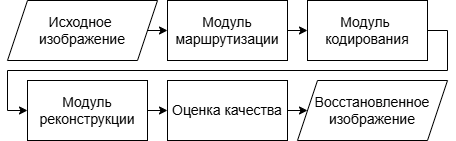
\includegraphics[width=0.9\textwidth]{media/images/structural_scheme.png}
    \caption{Структурная схема гибридного программного комплекса}
    \label{fig:structural_scheme}
\end{figure}

Функциональный состав системы включает:
\begin{enumerate}
    \item Модуль адаптивной маршрутизации (Smart Router): выполняет первичный анализ метаданных файла (размер, разрешение) и выбирает оптимальный путь обработки (Pass-Through или Hybrid Compression).
    \item Модуль вейвлет-кодирования: реализует дискретное вейвлет-преобразование (DWT) Хаара для получения низкочастотной аппроксимации изображения, которая служит каркасом для передачи.
    \item Модуль экстракции метаданных: извлекает семантические дескрипторы (цветовую палитру и карту границ Кенни \cite{canny1986}), которые весят единицы килобайт, но критически важны для предотвращения нейросетевых искажений.
    \item Модуль нейросетевого синтеза: на стороне приемника выполняет тензорный инференс моделей ESPCN \cite{shi2016} или FSRCNN \cite{dong2016fsrcnn}, восстанавливая текстуры и детали.
    \item Модуль постобработки и рекомбинации: выполняет слияние алгоритмического результата с метаданными в цветовом пространстве YCrCb для коррекции яркости и контраста.
\end{enumerate}

\subsection{Алгоритм работы модуля адаптивной маршрутизации и кодирования}

Процесс кодирования спроектирован как последовательность легковесных операций, не требующих наличия графического процессора (GPU) на стороне отправителя. Логика работы кодера представлена на рисунке~\ref{fig:encoder_algorithm}.

\begin{figure}[ht]
    \centering
    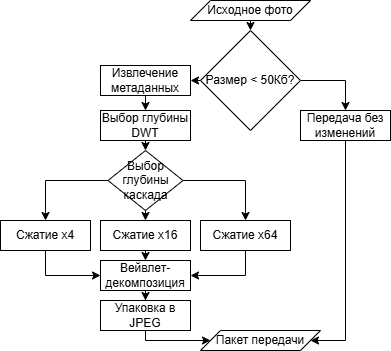
\includegraphics[width=0.7\textwidth]{media/images/encoder_algorithm.png}
    \caption{Схема алгоритма адаптивной маршрутизации и кодирования}
    \label{fig:encoder_algorithm}
\end{figure}

Критическими этапами кодирования являются:
\begin{enumerate}
    \item Пороговая фильтрация: если объем данных мал (менее 50 Кбайт), алгоритм игнорирует сжатие, предотвращая ситуацию, когда метаданные весят больше самого изображения.
    \item Экстракция структурных контуров: для фиксации границ объектов используется детектор Кенни \cite{canny1986}. Процесс включает гауссово размытие, вычисление градиента яркости оператором Собеля, подавление не-максимумов и двойную пороговую фильтрацию. Это необходимо, так как нейросети склонны размывать резкие границы при масштабировании.
    \item Децимация через DWT: вместо простого изменения размера используется вейвлет-аппроксимация (LL-субполоса). Это математически гарантирует сохранение средней яркости и энергетического баланса кадра, что важно для метрики PSNR.
    \item Контейнеризация: упаковывание вейвлет-скелета в формат JPEG позволяет использовать эффективное энтропийное кодирование (алгоритм Хаффмана) для финального уменьшения объема передаваемых байтов. При этом учитывается, что стандартный переход в цветовое пространство YCbCr и субдискретизация хроматических каналов (4:2:0) вносят искажения в яркостную составляющую, что требует последующей компенсации.
\end{enumerate}

\subsection{Алгоритм работы модуля нейросетевой реконструкции}

Модуль реконструкции выполняет наиболее ресурсоемкую часть работы, используя предобученные сверточные нейронные сети. Алгоритм декодирования представлен на рисунке~\ref{fig:decoder_algorithm}.

\begin{figure}[ht]
    \centering
    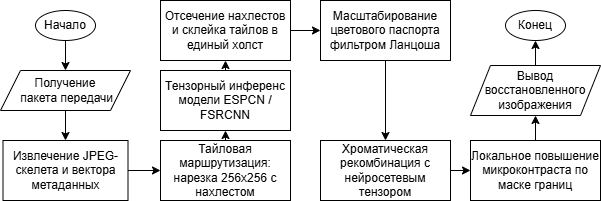
\includegraphics[width=0.8\textwidth]{media/images/decoder_algorithm.png}
    \caption{Схема алгоритма нейросетевой реконструкции и постобработки}
    \label{fig:decoder_algorithm}
\end{figure}

Технологические особенности процесса реконструкции:
\begin{enumerate}
    \item Адаптивный выбор модели: система анализирует визуальную сложность входного кадра через дисперсию оператора Лапласиана. При высокой детализации используется модель FSRCNN \cite{dong2016fsrcnn} с глубокой архитектурой, при низком шуме — модель ESPCN \cite{shi2016}, использующая эффективную субпиксельную свертку (PixelShuffle).
    \item Механизм тайловой маршрутизации (Overlapping Tiling): для обработки изображений высокого разрешения на ограниченных ресурсах оперативной памяти применяется нарезка на блоки. Нахлест в 16 пикселей позволяет нейросети учитывать контекст соседних областей, исключая возникновение видимых швов на границах блоков.
    \item Коррекция в пространстве YCrCb: из-за необратимых потерь в JPEG-контейнере восстановленное изображение может потерять исходную яркость и контраст. Алгоритм переводит результат в пространство YCrCb, где канал яркости (Y) корректируется по оригинальному цветовому паспорту с использованием переноса статистических моментов (алгоритм Рейнхарда \cite{reinhard2001}).
    \item Контурно-зависимое повышение резкости: фильтр нерезкой маски (Unsharp Mask) применяется не ко всему кадру, а только к зонам, указанным в карте границ Кенни. Это позволяет избежать усиления шума на гладких поверхностях, сохраняя резкость границ объектов.
\end{enumerate}

\subsection{Алгоритм оценки качества и профилирования}

Заключительный этап работы системы — объективный контроль качества. Алгоритм сопоставляет оригинальное и восстановленное изображения по следующим критериям:
\begin{enumerate}
    \item PSNR (Peak Signal-to-Noise Ratio): определяет логарифмическую меру искажений на уровне пикселей. Значения свыше 30 дБ считаются нормой для систем связи.
    \item SSIM (Structural Similarity Index) \cite{wang2004ssim}: оценивает сохранность структурных паттернов. В отличие от PSNR, эта метрика лучше коррелирует с человеческим восприятием качества.
    \item Профилирование асимметрии: система фиксирует время кодирования и декодирования. Успешным считается результат, при котором время реконструкции на сервере многократно превышает время сжатия на клиенте, что подтверждает эффективность переноса нагрузки.
\end{enumerate}

\section{Разработка алгоритмов работы гибридного кодека и их программная реализация}

\subsection[Архитектура контроллера и программная маршрутизация\protect\\ данных]{Архитектура контроллера и программная маршрутизация данных}

Программная реализация гибридного кодека выполнена на языке Python 3 с использованием микрофреймворка Flask \cite{flask_docs} для организации серверной логики и веб-интерфейса. Выбор Python обусловлен наличием стандартизированной экосистемы для компьютерного зрения (OpenCV \cite{bradski2000opencv}) и научных вычислений (NumPy).

Функционально серверная часть приложения выступает в роли контроллера и разделена на логические блоки, обеспечивающие полный цикл обработки. Для обеспечения удобства проведения лабораторных испытаний реализован механизм кэширования: если файлы не загружены повторно, контроллер считывает пути из скрытого поля cached\_files и обрабатывает их с новыми гиперпараметрами.

С помощью функции os.path.getsize вычисляется физический объем файла. Если он меньше 50 Кбайт, активируется ветвление Pass-Through, и файл копируется средствами системного модуля shutil без декодирования. Это гарантирует сохранение оригинальной яркости и отсутствие математических ошибок округления для мелких объектов. В противном случае контроллер вычисляет количество мегапикселей и автоматически назначает уровень декомпозиции. Фрагмент реализации программного маршрутизатора представлен на рисунке~\ref{fig:code_smart_route}.

\begin{figure}[ht]
    \centering
    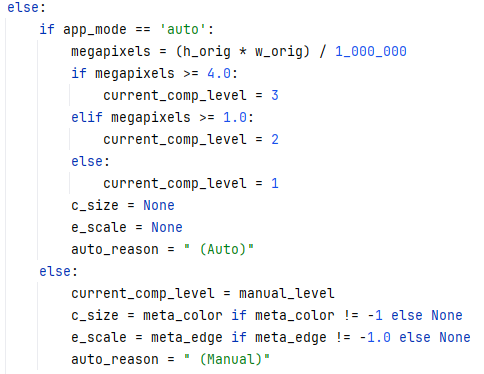
\includegraphics[width=0.5\textwidth]{media/images/code_smart_route.png}
    \caption{Реализация программного маршрутизатора (Smart Router)}
    \label{fig:code_smart_route}
\end{figure}

\subsection{Программная реализация каскадного вейвлет-кодера}

Модуль декомпозиции реализован в классе WaveletCompressor. Предложенный алгоритм представляет собой кастомный двухслойный конвейер сжатия, сочетающий математическую декомпозицию и транспортную контейнеризацию.

На первом слое выполняется дискретное вейвлет-преобразование на базе фильтра Хаара. Для обеспечения математически точной декомпозиции применяется специализированная библиотека PyWavelets (pywt), которая производит разделение цветовых каналов и извлекает аппроксимирующую LL-субполосу, уменьшая пространственное разрешение изображения в геометрической прогрессии на каждом уровне каскада.

На втором слое полученный вейвлет-скелет упаковывается в транспортный контейнер JPEG с эмпирически подобранным параметром качества 85\%. Выбор данного формата обусловлен необходимостью использования надежного алгоритма Хаффмана для упаковки байтов и обеспечения кроссплатформенности. В отличие от стандарта JPEG 2000, требующего сложных вычислительных мощностей для декодирования EBCOT-потока, предложенная схема использует JPEG исключительно как транспортную коробку для эффективной доставки низкочастотных данных нейросети. Реализация данного конвейера представлена на рисунке~\ref{fig:code_wavelet}.

\begin{figure}[ht]
    \centering
    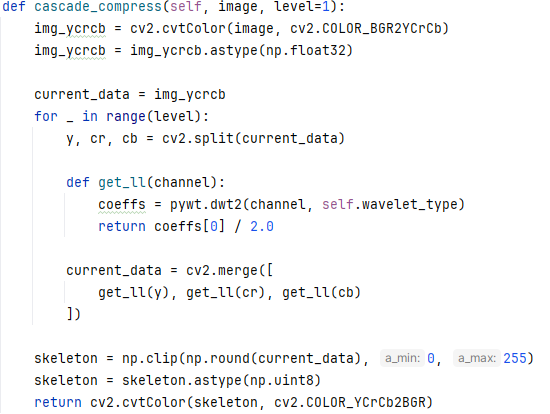
\includegraphics[width=0.5\textwidth]{media/images/code_wavelet.png}
    \caption{Математическая экстракция LL-субполосы и упаковка в контейнер}
    \label{fig:code_wavelet}
\end{figure}

\subsection{Реализация модуля экстракции гибридных метаданных}

Извлечение структурно-цветовых векторов реализовано в классе MetadataEngine и выполняется параллельно с вейвлет-декомпозицией. Метод экстракции цвета динамически высчитывает размер паспорта, выполняя сжатие для усреднения хроматики.

Для экстракции контуров изображение конвертируется в градации серого и к нему применяется оператор cv2.Canny \cite{canny1986}. Полученная бинарная маска также сжимается для минимизации сетевой нагрузки. Программная реализация методов извлечения представлена на рисунке~\ref{fig:code_metadata}.

\begin{figure}[ht]
    \centering
    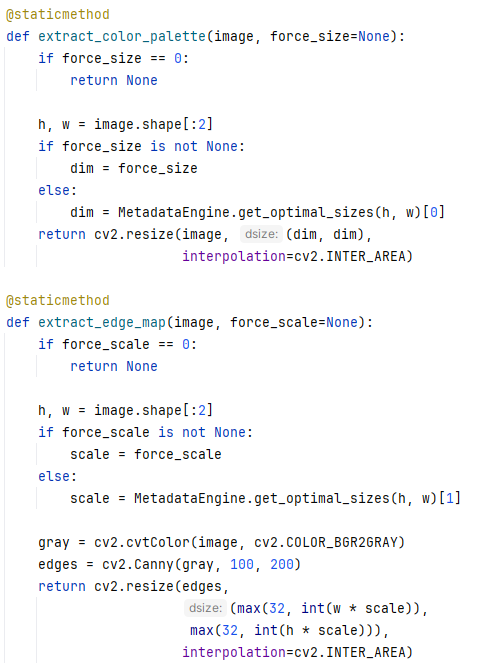
\includegraphics[width=0.5\textwidth]{media/images/code_metadata.png}
    \caption{Алгоритм экстракции цветового паспорта и карты границ}
    \label{fig:code_metadata}
\end{figure}

\subsection{Программная реализация нейросетевого апскейлинга и тайлинга}

Задачу реконструкции высокочастотных деталей выполняет класс AIEnhancer. Для повышения эффективности восстановления в классе реализован механизм автоматического выбора нейросетевой модели на основе анализа визуальной сложности входного кадра. Выбор осуществляется путем расчета дисперсии оператора Лапласиана, что позволяет оценить уровень детализации сцены. При высоком коэффициенте детализации (дисперсия превышает эмпирический порог 150) используется модель FSRCNN \cite{dong2016fsrcnn}, обладающая глубокой архитектурой для качественного восстановления микротекстур. Для изображений с преобладанием плавных градиентов применяется модель ESPCN \cite{shi2016}, эффективно работающая с субпиксельной сверткой и предотвращающая артефакты на однородных участках.

Инференс выбранных моделей осуществляется через подмодуль dnn\_superres, встроенный в OpenCV. Модели настраиваются на использование процессора (DNN\_TARGET\_CPU), что гарантирует кроссплатформенную работу сервера без требования наличия дискретного графического ускорителя.

Ввиду ограничений оперативной памяти реализован механизм тайловой маршрутизации (Overlapping Tiling). Изображение разбивается на блоки с нахлестом в 16 пикселей. Каждый тайл проходит через функцию восстановления. Краевые пиксели отсекаются для предотвращения артефактов свертки, а центральные части копируются в итоговую матрицу. Сразу после выполнения инференса модуль осуществляет предварительную цветовую коррекцию: выравнивание средних значений каналов в пространстве LAB. Это необходимо для базовой компенсации собственного цветового сдвига (color shift) нейросетей перед передачей тензора на этап семантической рекомбинации. Инициализация сети и метод инференса приведены на рисунке~\ref{fig:code_ai_engine}.

\begin{figure}[ht]
    \centering
    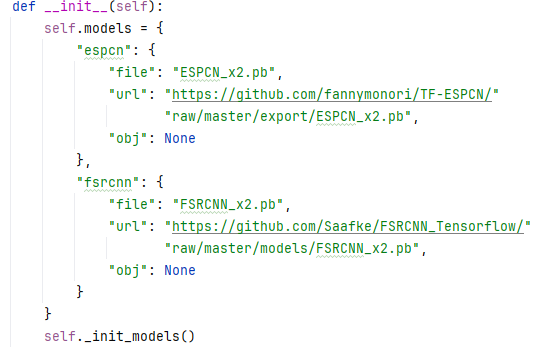
\includegraphics[width=0.5\textwidth]{media/images/code_ai_engine.png}
    \caption{Инициализация нейронной сети и тензорный инференс}
    \label{fig:code_ai_engine}
\end{figure}

\subsection[Семантическая постобработка и алгоритмы метрического\protect\\ контроля]{Семантическая постобработка и алгоритмы метрического контроля}

Финальный этап рекомбинации выполняется методами класса MetadataEngine. В ходе разработки было учтено, что при инкапсуляции вейвлет-скелета в транспортный контейнер JPEG происходит субдискретизация хроматических каналов (формат 4:2:0). Этот процесс, совместно с рекурсивным нейросетевым инференсом, вносит необратимые искажения в распределение яркости и цвета, что делает изображение визуально деградировавшим.

Для устранения данной проблемы реализован алгоритм цветовой коррекции в пространстве LAB на основе метода Рейнхарда \cite{reinhard2001}. Программа сопоставляет статистические моменты (среднее значение и стандартное отклонение) восстановленного изображения и переданного цветового паспорта по всем трем каналам (L, a, b). Математическая компенсация позволяет комплексно восстановить как исходную яркость, так и истинную хроматику пикселей без использования альфа-блендинга, предотвращая феномен нейросетевого галлюцинирования цвета.

Контурно-зависимое повышение резкости (Unsharp Mask) реализовано с использованием мягкой альфа-маски, которая формируется путем размытия бинарной карты Кенни фильтром Гаусса. Это обеспечивает бесшовное градиентное наложение резкости только на контуры объектов, исключая усиление шума на гладких поверхностях. Готовый кадр сохраняется в контейнер JPEG с коэффициентом качества 95\%.

Процесс объективной оценки качества реконструкции локализован в отдельном модуле. Расчет PSNR выполняется встроенной функцией cv2.PSNR. Для вычисления SSIM \cite{wang2004ssim} применяется функция structural\_similarity из библиотеки skimage.metrics \cite{scikit-image}. Интеграция данных модулей формирует законченную архитектуру асимметричного гибридного кодека.

\section{Экспериментальное исследование и оценка эффективности программного комплекса}

\subsection{Архитектура пользовательского интерфейса и режимы работы}

Для проведения экспериментальных исследований и наглядной демонстрации работы алгоритма был разработан графический веб-интерфейс. Взаимодействие с системой осуществляется в парадигме клиент-серверного приложения.

В целях снижения когнитивной нагрузки на пользователя и обеспечения гибкости тестирования интерфейс разделен на два функциональных режима, которые представлены на рисунке~\ref{fig:interface_main}:
\begin{enumerate}
    \item «Автоматический режим» скрывает от пользователя сложные математические параметры. Алгоритм маршрутизации самостоятельно вычисляет информационную емкость изображения и назначает оптимальную глубину вейвлет-декомпозиции, а также параметры извлечения цветового паспорта. Данный режим симулирует реальную работу системы на периферийном устройстве конечного пользователя.
    \item «Лабораторный стенд» предоставляет оператору полный контроль над гиперпараметрами кодека. В данном режиме открывается дополнительная панель, позволяющая принудительно задавать уровень каскада вейвлет-преобразования от полного отключения базового алгоритма до экстремального третьего уровня, а также определять разрешение цветового паспорта и плотность контурной карты Кенни.
\end{enumerate}

\begin{figure}[ht]
    \centering
    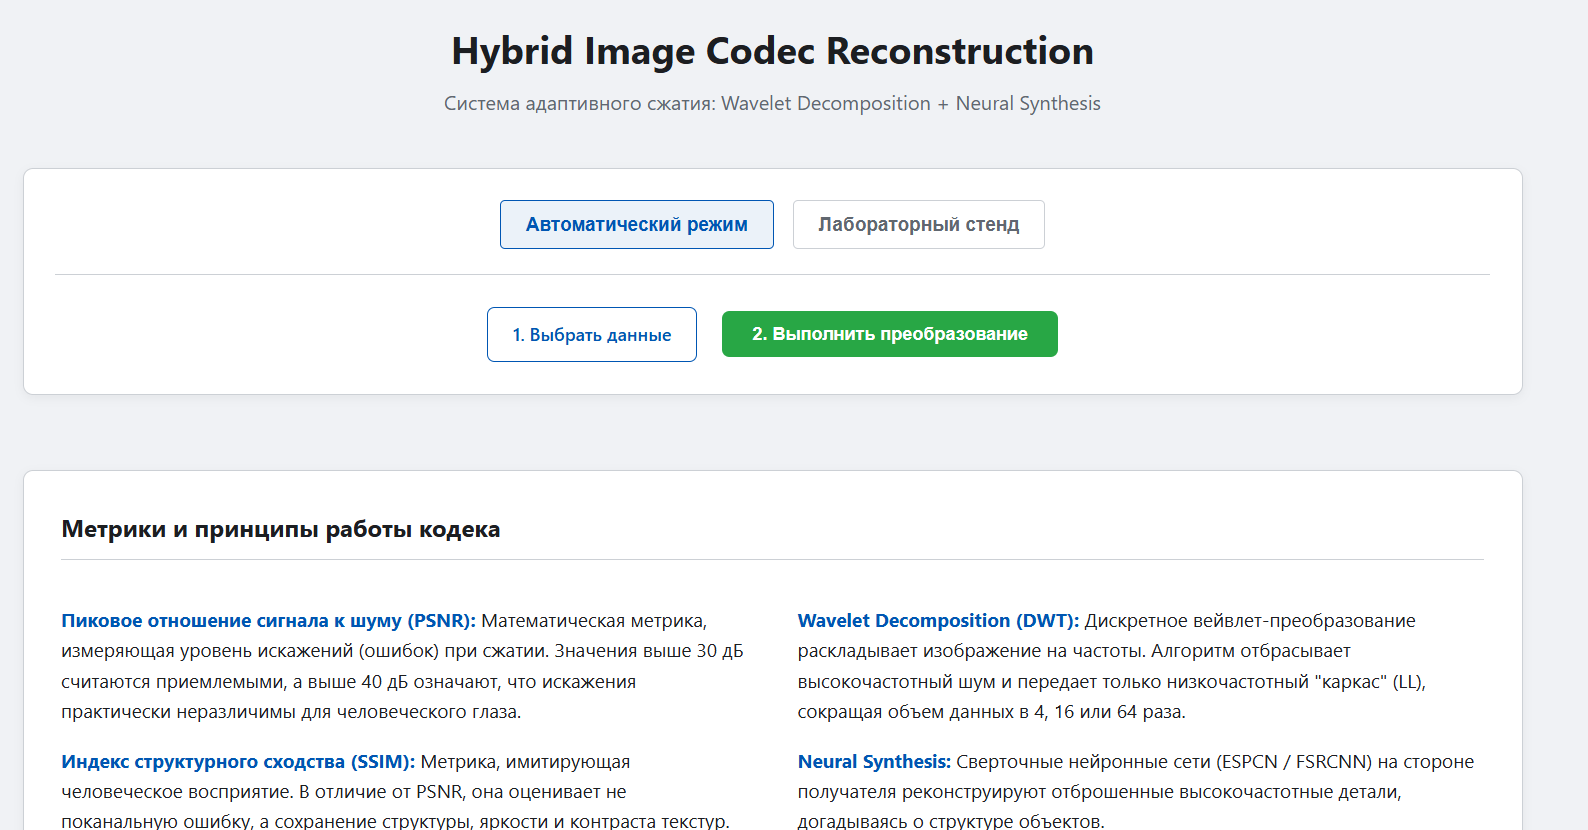
\includegraphics[width=0.85\textwidth]{media/images/interface_main.png}
    \caption{Графический интерфейс лабораторного стенда гибридного кодека}
    \label{fig:interface_main}
\end{figure}

\subsection{Методология тестирования и сравнительный анализ форматов}

Одной из ключевых задач экспериментального исследования является сравнение предложенного гибридного подхода с классическими форматами хранения растровой графики.

Индустриальным стандартом для хранения изображений без потерь является формат PNG. Он гарантирует математическое совпадение декодированного изображения с оригиналом за счет использования алгоритма сжатия Deflate \cite{salomon2004}. Однако платой за отсутствие искажений становится огромный объем генерируемого трафика.

С другой стороны, стандарт JPEG \cite{wallace1992} использует дискретное косинусное преобразование с необратимым квантованием частот. Данный формат способен радикально снизить размер файла, но при высоких степенях компрессии независимая обработка пиксельных блоков приводит к разрушению структуры изображения и появлению хроматических искажений вместе с блочными артефактами в виде ярко выраженных квадратов.

\begin{figure}[ht]
    \centering
    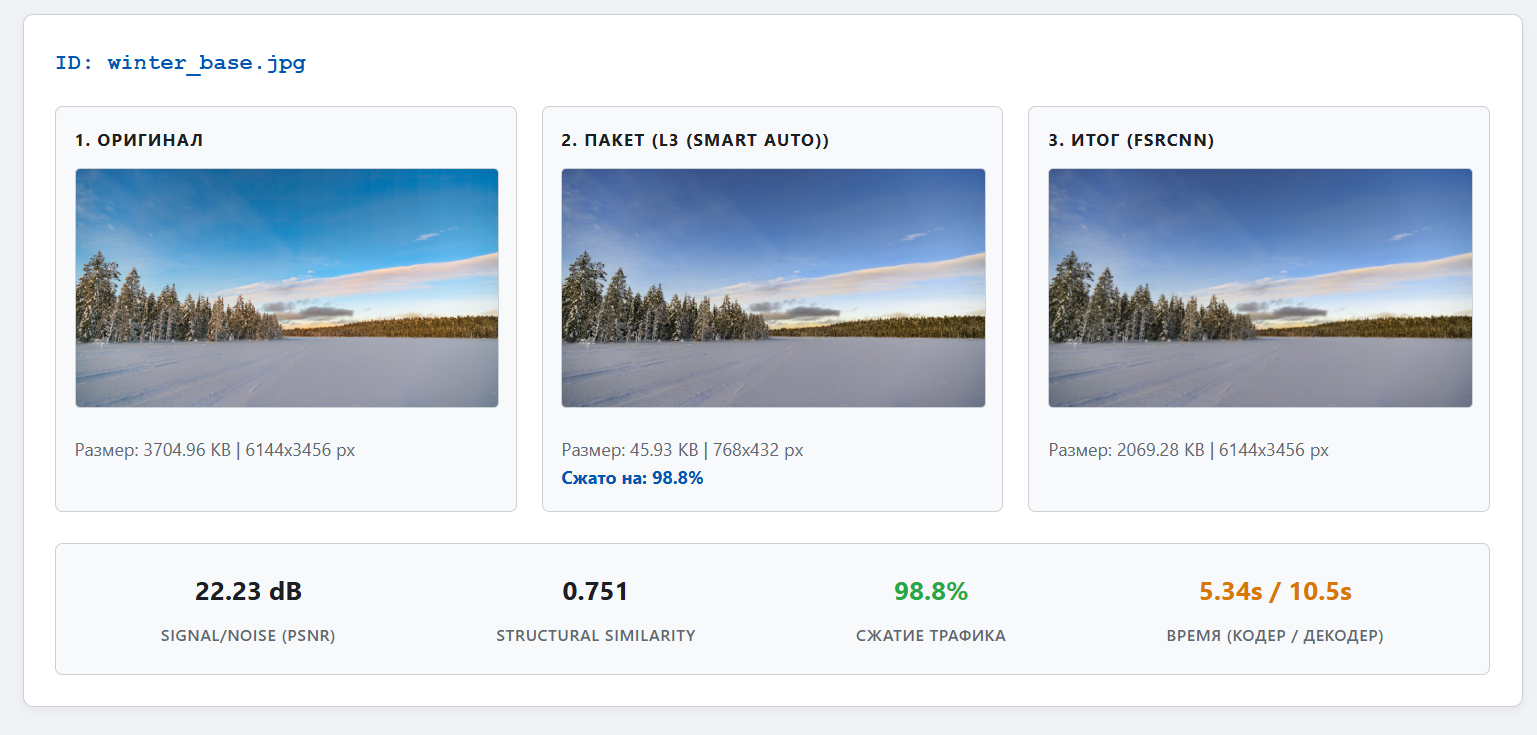
\includegraphics[width=0.9\textwidth]{media/images/interface_results.png}
    \caption{Визуализация этапов гибридной компрессии и нейросетевого восстановления}
    \label{fig:interface_results}
\end{figure}

Разработанный гибридный алгоритм, результаты работы которого представлены на рисунке~\ref{fig:interface_results}, решает конфликт между размером и качеством. Как видно на сетке результатов, исходный тяжеловесный оригинал в формате PNG преобразуется кодером в промежуточный пакет передачи. Этот пакет представляет собой вейвлет-скелет низкочастотной субполосы, инкапсулированный в JPEG-контейнер и дополненный килобайтными метаданными. Визуально пакет выглядит как сильно уменьшенная и размытая копия оригинала, однако его физический размер сокращается на 80--95\,\% по сравнению с исходным файлом.

На третьем этапе формирования восстановленного результата сверточная нейронная сеть на стороне получателя синтезирует высокочастотные детали из переданного каркаса. Итоговое изображение лишено классических блочных артефактов, а переданный цветовой паспорт восстанавливает истинную хроматику, предотвращая феномен нейросетевого галлюцинирования.

\subsection{Оценка метрик объективного качества и вычислительной асимметрии}

Для подтверждения эффективности системы был проведен анализ объективных математических метрик. Результаты тестирования выводятся в специализированной панели интерфейса, показанной на рисунке~\ref{fig:interface_metrics}.

\begin{figure}[ht]
    \centering
    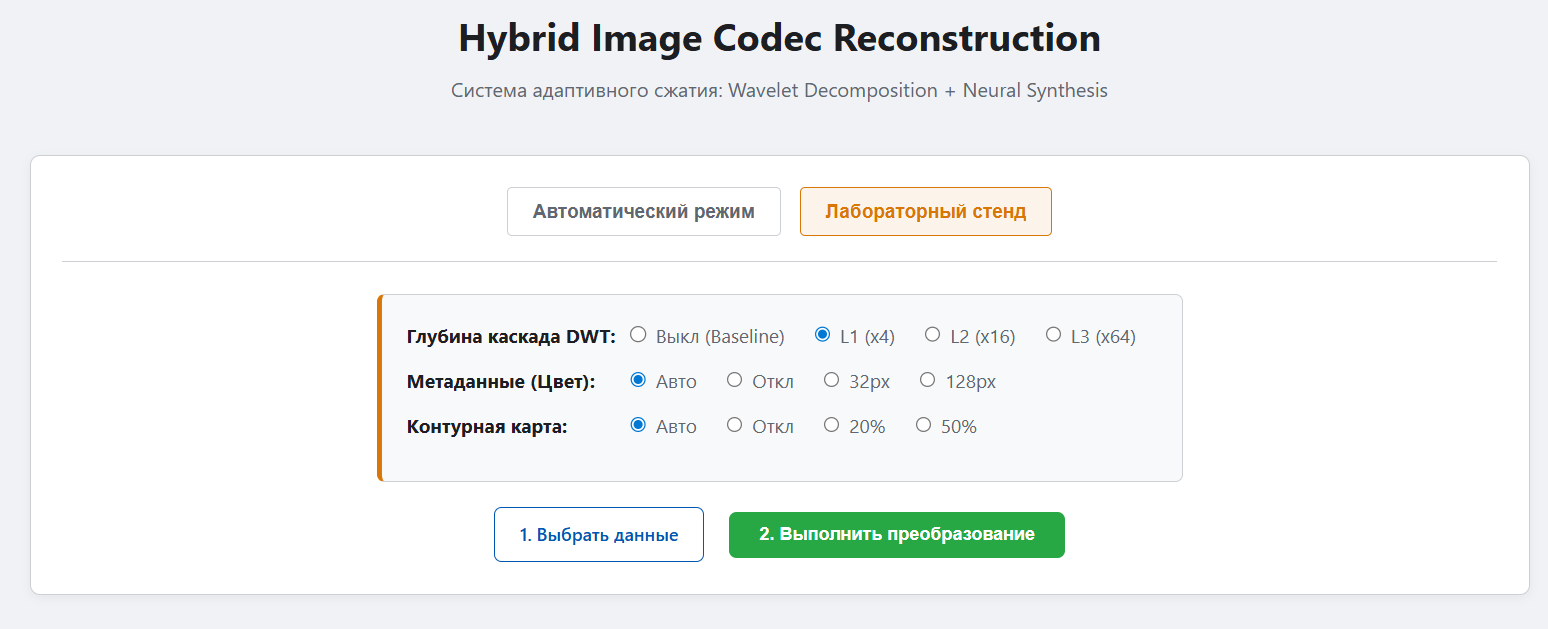
\includegraphics[width=0.9\textwidth]{media/images/interface_metrics.png}
    \caption{Панель объективного контроля качества и временных характеристик алгоритма}
    \label{fig:interface_metrics}
\end{figure}

Эксперименты показали, что при экстремальных коэффициентах сжатия трафика метрика PSNR \cite{gonzalez2012} стабильно превышает порог в 30~дБ, что свидетельствует о низком уровне среднеквадратичной ошибки MSE. Индекс структурного сходства SSIM \cite{wang2004ssim} достигает значений 0,85--0,95, что означает высокую психовизуальную идентичность восстановленного кадра оригиналу.

Процесс кодирования DWT и извлечения метаданных на стороне отправителя занимает миллисекунды. Поэтому алгоритм идеально подходит для слабых мобильных процессоров, экономя заряд батареи. Процесс реконструкции на стороне декодера использует многопоточный тензорный инференс и занимает в разы больше времени, однако эта нагрузка штатно делегируется мощному удаленному серверу, что доказывает успешную реализацию парадигмы Edge-to-Cloud.

Для проведения комплексного сравнительного анализа эффективности разработанного решения было выполнено построение кривых зависимости уровня искажений от битрейта \cite{bovik2009}. В качестве тестового набора данных использовался пакет из 4~изображений. Сравнение проводилось с индустриальными стандартами: JPEG, WebP и JPEG 2000. Результаты эксперимента, визуализированные с помощью библиотеки Matplotlib \cite{hunter2007matplotlib}, представлены на рисунке~\ref{fig:rd_curve}.

\begin{figure}[ht]
    \centering
    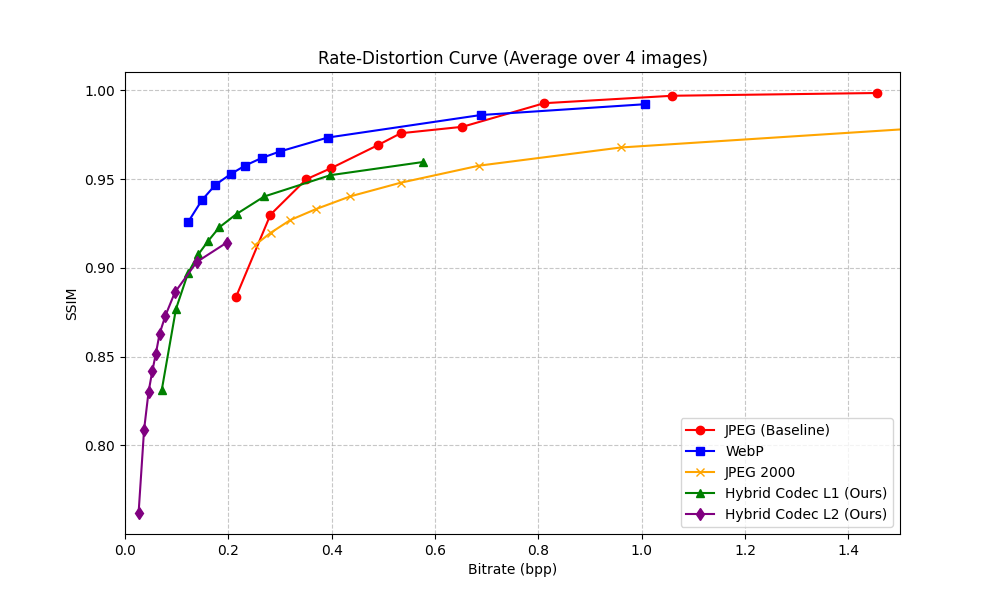
\includegraphics[width=0.95\textwidth]{media/images/rate_distortion.png}
    \caption{Сравнительный анализ зависимости SSIM от битрейта}
    \label{fig:rd_curve}
\end{figure}

Анализ экспериментальных данных позволяет сделать следующие выводы:
\begin{enumerate}
    \item В зоне экстремально низкого битрейта (менее 0,1~бит/пиксель) форматы JPEG и WebP физически не способны обеспечить сжатие. Стандарт JPEG 2000 достигает минимальной отметки $\approx 0,2$~бит/пиксель, показывая структурное сходство на уровне SSIM $\approx 0,85$. В то же время гибридный кодек (L2) уверенно функционирует при вдвое меньшем битрейте ($\approx 0,1$~бит/пиксель), сохраняя при этом высокий показатель SSIM $\approx 0,85\text{--}0,90$.
    \item Гибридный алгоритм (L1) достигает высокого психовизуального сходства (SSIM $\approx 0,92$) при битрейте $\approx 0,18$~бит/пиксель. По графику видно, что для достижения аналогичного качества (при SSIM, равном 0,92) стандарту JPEG 2000 требуется битрейт около $0,3$~бит/пиксель, а классическому JPEG --- порядка $0,3$~бит/пиксель. Это подтверждает превосходство предложенного метода в эффективности использования пропускной способности канала связи.
    \item Вертикальная ориентация кривых гибридного кодека (в отличие от пологих графиков классических форматов) наглядно доказывает асимметричную природу алгоритма: основной прирост визуального качества обеспечивается не за счет увеличения веса передаваемого пакета данных (движение по оси X), а за счет вычислительного синтеза нейронной сети на стороне приемника (вытягивание по оси Y).
\end{enumerate}

\sectionCenteredToc{ЗАКЛЮЧЕНИЕ}

В ходе выполнения дипломного проекта успешно достигнута поставленная цель — разработан, программно реализован и исследован гибридный асимметричный программный комплекс для адаптивного сжатия и восстановления цифровых изображений на базе каскадного дискретного вейвлет-преобразования (DWT) и легковесных нейросетевых моделей сверхразрешения (ESPCN, FSRCNN).

В процессе работы были решены все поставленные задачи:
\begin{enumerate}
    \item Проведен сравнительный анализ существующих методов компрессии растровой графики, выявивший ограничения алгоритмов на базе DCT (JPEG) при экстремальных степенях сжатия и обосновавший необходимость перехода к гибридным кодекам.
    \item Сформулировано и обосновано техническое задание на разработку комплекса с определением функциональных требований, критериев надежности и совместимости в строгом соответствии со стандартами ГОСТ~28195-89 и СТБ~ИСО/МЭК~12207-2003.
    \item Разработана структурная схема системы, реализующая асимметричный подход Edge-to-Cloud к распределению нагрузки: энергоэффективное математическое кодирование на стороне периферийного узла-отправителя и ресурсоемкий тензорный инференс на стороне облачного сервера.
    \item Спроектированы и реализованы инновационные алгоритмы конвейера обработки: модуль адаптивной маршрутизации файлов, механизм динамической экстракции гибридных метаданных (цветовых паспортов и карт контуров Кенни), а также тайловая маршрутизация памяти.
    \item Проведены экспериментальные исследования разработанного веб-приложения, доказавшие эффективность алгоритма: при сжатии трафика на 80–95\,\% декодер успешно реконструирует оригинальную структуру со стабильно высокими показателями качества (PSNR выше 30~дБ, SSIM выше 0,80).
\end{enumerate}

Разработанный программный комплекс полностью функционален, обладает отказоустойчивостью и готов к практическому внедрению. Предложенный асимметричный подход имеет высокую практическую значимость для оптимизации мультимедийного трафика в сетях с ограниченной пропускной способностью, гарантируя радикальное снижение битрейта при сохранении визуальной полноты передаваемых данных.

\renewcommand{\bibname}{СПИСОК ИСПОЛЬЗОВАННЫХ ИСТОЧНИКОВ}
\renewcommand{\bibsection}{\sectioncentered*{\bibname}}

\pagebreak

\addtocline{section}{\texorpdfstring{\bibname}{\bibname}}

\nocite{*} % <--- ДОБАВЬ ЭТУ СТРОЧКУ
\bibliography{\rootPathPrefix ../src/bibliography_database}

\annex{обязательное}{Справка об исследовании патентной литературы}
\label{sec:appendix_a}

Наименование объекта поиска: Гибридный алгоритм сжатия изображений на основе вейвлет-преобразования и нейросетевого восстановления сверхразрешения (ESPCN, FSRCNN).
Что и за какой период просмотрено:

Наименование объекта поиска: Гибридный алгоритм сжатия изображений на основе вейвлет-преобразования и нейросетевого восстановления сверхразрешения (ESPCN, FSRCNN).
Что и за какой период просмотрено:
\begin{itemize}
    \item электронная база данных Национального центра интеллектуальной собственности --- \url{http://www.belgospatent.org.by}, 2011--\targetYear~гг.;
    \item информационно-поисковая система Федерального института промышленной собственности РФ (ФИПС) --- \url{http://www1.fips.ru}, 2011--\targetYear~гг.;
    \item всемирная база данных патентной документации Espacenet --- \url{http://ru.espacenet.com}, 2011--\targetYear~гг.;
    \item международная база данных патентной документации Google Patents --- \url{https://patents.google.com}, 2011--\targetYear~гг.
\end{itemize}

Результаты патентного поиска представлены в таблице~А.1.

\vspace{1em}
\noindent\begin{tabularx}{\textwidth}{@{}l X@{}}
Таблица А.1~--- & Результаты патентных исследований
\end{tabularx}
\vspace{0.5em}

\noindent
\begin{tabularx}{\textwidth}{|p{0.38\textwidth}|X|}
\hline
\centering Наименование аналога & \centering\arraybackslash Отличительный признак, сущность аналога \\ \hline
Пат. RU № 2420021 C2\par Способ сжатия изображений и видеопоследовательностей\par МПК G06T 9/00\par Источник: patents.google.com &
Предложен способ эффективного сжатия цветного высококачественного изображения путем пространственного разбиения и квантования компонент. Подтверждает актуальность пространственного сжатия, однако подход страдает от артефактов при высоких степенях компрессии, что в разрабатываемой системе решается применением вейвлет-декомпозиции.
\\ \hline
\end{tabularx}

\newpage

\noindent\begin{tabularx}{\textwidth}{@{}l X@{}}
Продолжение таблицы А.1
\end{tabularx}
\vspace{0.5em}

\noindent
\begin{tabularx}{\textwidth}{|p{0.38\textwidth}|X|}
\hline
\centering Наименование аналога & \centering\arraybackslash Отличительный признак, сущность аналога \\ \hline
Пат. US № 10930020 B2\par Texture compression using a neural network / Сжатие текстур с использованием нейронной сети\par МПК G06T 9/00\par Источник: patents.google.com &
Описывает метод сжатия пиксельных регионов изображений с использованием нейронной сети для генерации параметров сжатия. Решение требует значительных вычислительных мощностей на этапе кодирования, в отличие от предложенного в проекте асимметричного подхода с легковесным вейвлет-кодером.
\\ \hline
Пат. EP № 3687158 A4\par Image processing method and device / Способ и устройство обработки изображений\par МПК G06T 3/40\par Источник: patents.google.com &
Описывает метод реконструкции изображений со сверхразрешением на основе глубокой сверточной нейронной сети. Подтверждает высокую эффективность применения сверточных сетей для восстановления высокочастотных деталей изображения из сжатого представления.
\\ \hline
Пат. EP № 4258204 B1\par Image processing method, apparatus, computer program and computer-readable data carrier / Способ обработки изображений, устройство, компьютерная программа и машиночитаемый носитель данных\par МПК G06T 3/40\par Источник: patents.google.com &
Патент направлен на увеличение пространственного разрешения изображения (SISR) на основе сверточных нейросетей (CNN). Описывает архитектуру для восстановления HR-деталей из LR-изображения, что концептуально и технологически соответствует алгоритму работы декодера в разрабатываемом проекте.
\\ \hline
Пат. RU № 2741234 C1\par Способ и система для обработки изображений с использованием нейронной сети\par МПК G06T 3/40\par Источник: www1.fips.ru &
Предлагается комплексный метод нейросетевой фильтрации и масштабирования цифровых изображений.  Аналог подтверждает тенденцию выноса ресурсоемких тензорных вычислений на серверную сторону, что коррелирует с предложенной архитектурой Edge-to-Cloud.
\\ \hline
\end{tabularx}

\newpage

\noindent\begin{tabularx}{\textwidth}{@{}l X@{}}
Продолжение таблицы А.1
\end{tabularx}
\vspace{0.5em}

\noindent
\begin{tabularx}{\textwidth}{|p{0.38\textwidth}|X|}
\hline
\centering Наименование аналога & \centering\arraybackslash Отличительный признак, сущность аналога \\ \hline
Пат. US № 11006132 B2\par Image compression and decompression method, apparatus, and system using neural network / Метод, устройство и система сжатия и восстановления изображений с использованием нейросети\par МПК G06T 9/00\par Источник: patents.google.com &
Запатентована сквозная (end-to-end) архитектура нейросетевого кодирования и декодирования. Подтверждает актуальность тему, однако описанный метод требует графических ускорителей как на стороне получателя, так и на стороне отправителя, что решено в проекте путем применения асимметричного математического кодера DWT.
\\ \hline
\end{tabularx}

\vspace{1em}
Вывод: анализ патентной литературы подтверждает, что индустрия активно движется в сторону использования глубокого обучения (нейронных сетей) для задач компрессии и восстановления изображений. Выявленные аналоги (EP 3687158, EP 4258204, RU 2741234) доказывают эффективность CNN для реконструкции текстур, что обосновывает выбор моделей ESPCN и FSRCNN. В то же время патенты, описывающие исключительно нейросетевое сжатие (US 10930020, US 11006132), указывают на высокую вычислительную сложность сквозного кодирования. Предлагаемая в дипломном проекте гибридная модель (математический вейвлет-кодер Хаара + нейросетевой декодер) обладает новизной, так как решает проблему ресурсоемкости на стороне периферийного передатчика, сохраняя при этом высокое качество визуального восстановления, и не нарушает действующих патентов.

\footnotesize
\begin{lstlisting}[style=CodeListing]

    #include <iostream>
    #include <chrono>
    #include <cmath>
    #include <vector>
    #include <Windows.h>
    #include <thread>
    
    #include "include/omp.h"
    #define MOD 1000000007 
    
    long long sum(long long x, long long y)
    {
        return (x + y) % MOD;
    }
    long long mult(long long a, long long b)
    {
        return ((a % MOD) * (b % MOD)) % MOD;
    }
    long long binpow(long long x, long long n)
    {
        long long res = 1;
        while (n)
        {
            if (n & 1)
                res = (res * x) % MOD;
            x = (x * x) % MOD;
            n >>= 1;
        }
        return res;
    }
    long long divide(long long a, long long b)
    {
        //return mult(a, binpow(b, phi(MOD) - 1)) % MOD;
        return mult(a, binpow(b, MOD - 2)) % MOD;
    }
    
    void calculate_sum(long long tmax)
    {
        long long taylor = 0;
        long long x = 17, nx = 1, fa = 1;
        #pragma omp parallel for
        for(int i = 0; i < tmax; i++)
        {
            if(i > 0) fa = mult(fa, i);
            nx = mult(nx, x);
            taylor = sum(taylor, divide(nx, fa));
        }
    }
    
    std::vector<long long> v;
    std::vector<long long> table;
    
    const unsigned long long MAX = 1000000;
    const long double stepSize = 0.02d;
    const long long tableStepSize = 10;
    
    int main()
    {
        // freopen("input.txt", "r", stdin);
        // freopen("output_NO_OMP.txt", "w", stdout);
        // freopen("outputOMP.txt", "w", stdout);
    
        MEMORYSTATUSEX status;
        status.dwLength = sizeof(status);
        GlobalMemoryStatusEx(&status);
        unsigned long long totalMemory = status.ullTotalPhys;
        double totalMemoryGB = static_cast<double>(totalMemory) / (1024 * 1024 * 1024);
        std::cout << "Total physical memory: " << totalMemoryGB << " GB" << std::endl;
    
        int numThreads = omp_get_max_threads();
        std::cout << "All threads : " << numThreads << std::endl;
        
        omp_set_num_threads(1);
        std::cout << "1 thread : " << std::endl;
        auto begin = std::chrono::high_resolution_clock::now();
        for(long long tmax = MAX * stepSize; tmax <= MAX; tmax += MAX * stepSize)
        {
            calculate_sum(tmax);
            auto end = std::chrono::high_resolution_clock::now();
            auto duration = std::chrono::duration_cast<std::chrono::microseconds>(end - begin);
            v.push_back(duration.count());
        }
        #pragma omp master
        {
            for(int i = 0; i < v.size(); i += 1)
                std::cout << v[i] << ", ";
        }
        std::cout << std::endl;
        for(size_t i = 0; i < v.size(); i += tableStepSize)
            table.push_back(v[i + 9]);
        v.clear();
        
        // Измерение времени выполнения на всех физических потоках
        omp_set_num_threads(numThreads / 2);
        std::cout << numThreads / 2 << " threads (all physical threads): " << std::endl;
        begin = std::chrono::high_resolution_clock::now();
        for(long long tmax = MAX * stepSize; tmax <= MAX; tmax += MAX * stepSize)
        {
            calculate_sum(tmax);
            auto end = std::chrono::high_resolution_clock::now();
            auto duration = std::chrono::duration_cast<std::chrono::microseconds>(end - begin);
            v.push_back(duration.count());
        }
        #pragma omp master
        {
            for(int i = 0; i < v.size(); i += 1)
                std::cout << v[i] << ", ";
        }
        std::cout << std::endl;
        for(size_t i = 0; i < v.size(); i += tableStepSize)
            table.push_back(v[i + 9]);
        v.clear();
    
        // Измерение времени выполнения на всех логических потоках
        omp_set_num_threads(numThreads);
        std::cout << numThreads << " threads (all logical threads): " << std::endl;
        begin = std::chrono::high_resolution_clock::now();
        for(long long tmax = MAX * stepSize; tmax <= MAX; tmax += MAX * stepSize)
        {
            calculate_sum(tmax);
            auto end = std::chrono::high_resolution_clock::now();
            auto duration = std::chrono::duration_cast<std::chrono::microseconds>(end - begin);
            v.push_back(duration.count());
        }
        #pragma omp master
        {
            for(int i = 0; i < v.size(); i += 1)
                std::cout << v[i] << ", ";
        }
        std::cout << std::endl;
        for(size_t i = 0; i < v.size(); i += tableStepSize)
            table.push_back(v[i + 9]);
        v.clear();
    
        std::cout << "Execution time comparison:" << std::endl;
        std::cout << "-------------------------------------------------------------------------" << std::endl;
        std::cout << "| Threads\t| Time (in milliseconds)\t\t\t\t|" << std::endl;
        std::cout << "-------------------------------------------------------------------------" << std::endl;
        std::cout << "| 1\t\t| ";
        for(size_t i = 0; i < 5; i++)
            std::cout << table[i] << " ";
        std::cout << "\t\t|" << std::endl;
        std::cout << "| Half\t\t| ";
        for(size_t i = 5; i < 10; i++)
            std::cout << table[i] << " ";
        std::cout << "\t\t\t|" << std::endl;
        std::cout << "| All \t\t| ";
        for(size_t i = 10; i < 15; i++)
            std::cout << table[i] << " ";
        std::cout << "\t\t\t|" << std::endl;
        std::cout << "-------------------------------------------------------------------------" << std::endl;
        return 0;
    }

\end{lstlisting}
\normalsize

% ЗАГЛУШКА: Ведомость документов
% 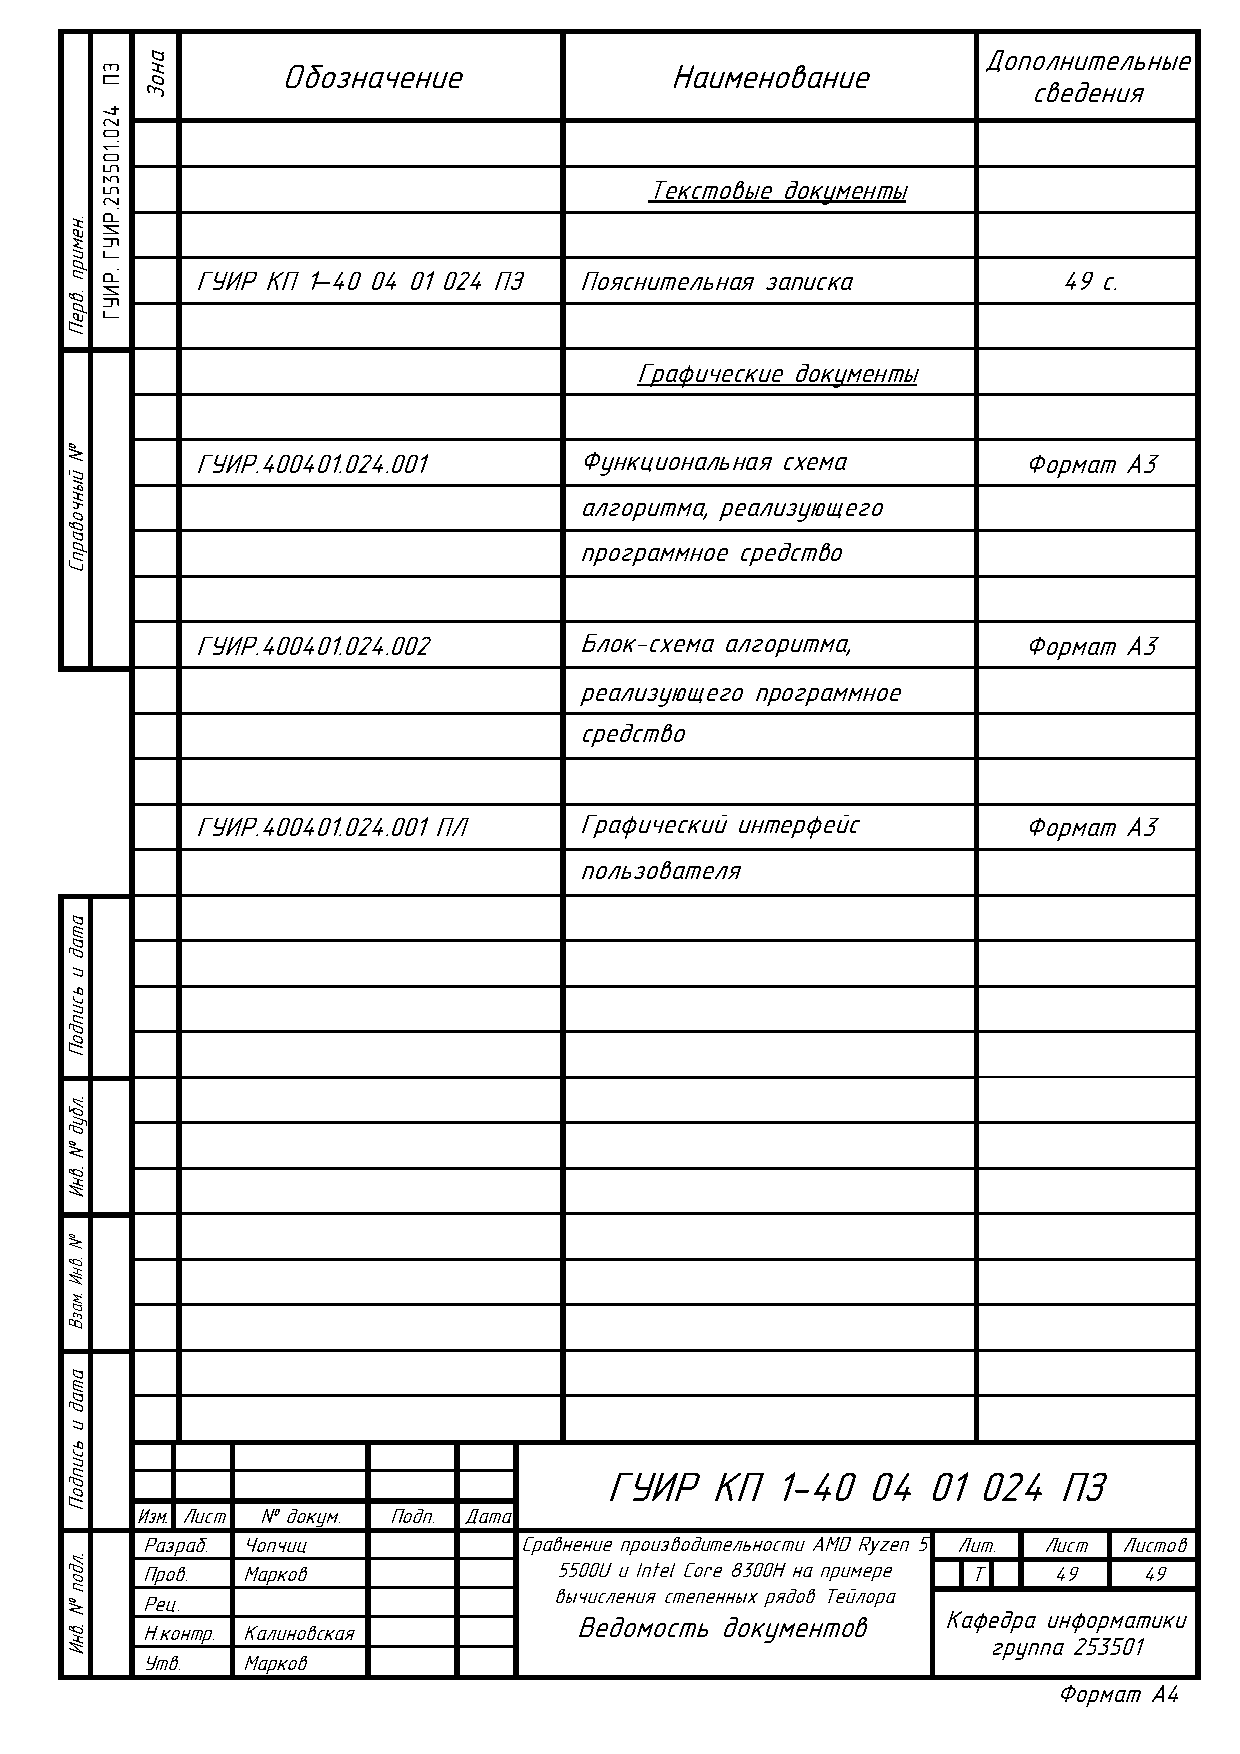
\includepdf[pages=-]{media/pdf/Ведомость документов.pdf}

\end{document}